%%%%%%%%%%%%%%%%%%%%%%% file template.tex %%%%%%%%%%%%%%%%%%%%%%%%%
%
% This is a general template file for the LaTeX package SVJour3
% for Springer journals.          Springer Heidelberg 2010/09/16
%
% Copy it to a new file with a new name and use it as the basis
% for your article. Delete % signs as needed.
%
% This template includes a few options for different layouts and
% content for various journals. Please consult a previous issue of
% your journal as needed.
%
%%%%%%%%%%%%%%%%%%%%%%%%%%%%%%%%%%%%%%%%%%%%%%%%%%%%%%%%%%%%%%%%%%%
%
% First comes an example EPS file -- just ignore it and
% proceed on the \documentclass line
% your LaTeX will extract the file if required
\begin{filecontents*}{example.eps}
%!PS-Adobe-3.0 EPSF-3.0
%%BoundingBox: 19 19 221 221
%%CreationDate: Mon Sep 29 1997
%%Creator: programmed by hand (JK)
%%EndComments

\end{filecontents*}
%
\RequirePackage{fix-cm}
%
\documentclass[final]{svjour3}                     % onecolumn (standard format)
%\documentclass[smallcondensed]{svjour3}     % onecolumn (ditto)
%\documentclass[smallextended]{svjour3}       % onecolumn (second format)
%\documentclass[twocolumn]{svjour3}          % twocolumn
%
\smartqed  % flush right qed marks, e.g. at end of proof
%
\usepackage[authoryear,comma]{natbib}
 \usepackage{mathptmx}      % use Times fonts if available on your TeX system
%
% insert here the call for the packages your document requires
\usepackage[pagebackref=true,colorlinks=true, linkcolor=blue,anchorcolor=blue,citecolor=blue,filecolor=blue,menucolor=blue,
urlcolor=cyan,plainpages=false,pdfpagemode=UseThumbs,pdftitle={Titre},pdfauthor={oluwole},
pdfsubject={Thesis},pdfstartview=FitH]{hyperref}% Extensions PDF
%\def\pdfBorderAttrs{/Border [0 0 0] } % Options PDF (No border around Links)
%\usepackage[plainpages=false,backref=page,hypertexnames=true,linktocpage=true,colorlinks=true,citecolor=blue,linkcolor=blue]{hyperref}
\usepackage{pdfpages}
%\usepackage{chicago}
\usepackage[onehalfspacing]{setspace}
%\doublespacing
%\linespread{1.6}
\setstretch{1.5}
\usepackage{apalike}
\onehalfspacing
\usepackage[left=40mm,right=25mm,top=30mm,bottom=20mm,headsep=10mm]{geometry}
\geometry{a4paper}
%\usepackage{amsmath}

\usepackage{amsmath,amsfonts,amssymb}

\usepackage{fancybox}
\usepackage{graphicx}
\usepackage{setspace}
%\usepackage[small]{caption}
\usepackage{color}
\usepackage{placeins}
\usepackage{epstopdf}
\usepackage{booktabs}
\usepackage{tikz}
\usepackage{subcaption}
%
% please place your own definitions here and don't use \def but
% \newcommand{}{}
%
 %Oluwole
 
\DeclareMathSymbol{\bLambda}{\mathalpha}{letters}{"03}
%\DeclareMathSymbol{\bGamma}{\mathalpha}{letters}{"00}
%\DeclareMathSymbol{\hbGamma}{\mathalpha}{letters}{"00}

\newcommand{\bt}{{\bf t}}
\newcommand{\bB}{{\bf B}}
%\newcommand{\b0}{{\bf 0}}
%%\newcommand{\b0}{{\boldsymbol{0}}}
\newcommand{\bSigma}{{\boldsymbol{\Sigma}}}
\newcommand{\tbSigma}{{\tilde {\boldsymbol{\Sigma}}}}
\newcommand{\tbu}{{\tilde {\bf u}}}
\newcommand{\tbU}{{\tilde {\bf U}}}
\newcommand{\bh}{{\bf h}}
\newcommand{\bH}{{\bf H}}
\newcommand{\bD}{{\bf D}}
\newcommand{\bU}{{\bf U}}
\newcommand{\bu}{{\bf u}}
\newcommand{\bZ}{{\bf Z}}
\newcommand{\bz}{{\bf z}}
\newcommand{\bC}{{\bf C}}
\newcommand{\bc}{{\bf c}}
%%
\newcommand{\bx}{{\bf x}}
\newcommand{\bX}{{\bf X}}
\newcommand{\by}{{\bf y}}
\newcommand{\bY}{{\bf Y}}
\newcommand{\bE}{{\bf E}}
\newcommand{\bW}{{\bf W}}
\newcommand{\tbx}{{\tilde {\bf x}}}
\newcommand{\tbX}{{\tilde {\bf X}}}
\newcommand{\tby}{{\tilde {\bf y}}}
\newcommand{\tbY}{{\tilde {\bf Y}}}
\newcommand{\hbX}{{\hat {\bf X}}}
\newcommand{\hbY}{{\hat {\bf Y}}}
\newcommand{\hby}{{\hat {\bf y}}}
\newcommand{\ty}{{\tilde {y}}}
\newcommand{\hy}{{\hat {y}}}
\newcommand{\bs}{{\bf s}}

\newcommand{\tC}{{\tilde {C}}}
\newcommand{\tP}{{\tilde {P}}}
\newcommand{\bK}{{\mathbf{K}}}
\newcommand{\bI}{{\mathbf{I}}}
\newcommand{\br}{{\mathbf{r}}}

%\newcommand{\bLambda}{\mathbf{\Lambda}}
\newcommand{\bGamma}{\mathbf{\Gamma}}
\newcommand{\hbGamma}{\hat {\mathbf{\Gamma}}}

\newcommand{\bgamma}{{\boldsymbol{\gamma}}}
\newcommand{\bepsilon}{{\boldsymbol{\varepsilon}}}
\newcommand{\tbepsilon}{{\tilde{\boldsymbol{\varepsilon}}}}
\newcommand{\hbepsilon}{{\hat{\boldsymbol{\varepsilon}}}}
\newcommand{\bbeta}{{\boldsymbol{\beta}}}
\newcommand{\hbbeta}{{\hat{\boldsymbol{\beta}}}}
\newcommand{\btau}{{{\boldsymbol{\tau}}}}
\newcommand{\balpha}{{\boldsymbol{\alpha}}}
\newcommand{\bhalpha}{{\hat{\boldsymbol{\alpha}}}}
\newcommand{\hbB}{{\hat{\boldsymbol{B}}}}
\newcommand{\hbSigma}{{\hat{\boldsymbol{\Sigma}}}}
\newcommand{\bmu}{{{\boldsymbol{\mu}}}}
%\newcommand{\bSigma}{{\mathbf{\Sigma}}}

%==========Divers===========:
\DeclareMathOperator*{\ssum}{{\textstyle \sum}}

% Insert the name of "your journal" with
 \journalname{Mathematical Biology}

%
\begin{document}
%
\title{Statistical emulation of Individual-based model simulation of microbial communities using cokriging
%\thanks{Grants or other notes
%about the article that should go on the front page should be
%placed here. General acknowledgments should be placed at the end of the article.}
}
%\subtitle{Do you have a subtitle?\\ If so, write it here}

%\titlerunning{Gaussian process emulator for upscaling complex multi-scale stochastic biological models}        % if too long for running head

\author{Oluwole K. Oyebamiji  \and Darren J. Wilkinson  \and
%Prashant Gupta \and
Jayathilake Gedara et al.
 }

%\authorrunning{Short form of author list} % if too long for running head

\institute{Newcastle University, School of Mathematics \& Statistics \at Newcastle upon Tyne, NE1 7RU, UK. \\
              Tel.: (+44) 7411875750\\
              %Fax: (+44) 1908 655 151\\
              \email{wolemi2@yahoo.com}           \\
%             \emph{Present address:} of F. Author\\
Darren J. Wilkinson  \\ 
Newcastle University, School of Mathematics \& Statistics \at Newcastle upon Tyne, NE1 7RU, UK. \\ 
Jayathilake Gedara \\
Newcastle University, Department of Mechanical \& Systems Engineering \at Newcastle upon Tyne, NE1 7RU, UK.\\
%Prashant Gupta ~\\% Steven Rushton \\
%Newcastle University, Department of Biology, \at Newcastle upon Tyne, NE1 7RU, UK.\\
}

\date{Received: date / Accepted: date}
% The correct dates will be entered by the editor


\maketitle

\begin{abstract}
The performance of credible simulations in open engineered biological frameworks is an important step for practical application of scientific knowledge to solve real-world problems and enhance our ability to make novel discoveries. Therefore, maximising our potential to explore the range of solutions at frontier level could reduce the potential risk of failure on a large scale. One primary application of this type of knowledge is in the management of wastewater treatment systems. Efficient optimisation of wastewater treatment plant focuses on aggregate outcomes of individual particle-level processes. One of the crucial aspects of engineering biology approach in wastewater treatment study is to run a high complex simulation of biological particles. This type of model can scale from one level to another and can also be used to study how to manage real systems effectively with minimal physical experimentation. 

Nevertheless, simulation of open biological systems is challenging because they often involve a large number of bacteria that ranges from order $10^{12}$ to $10^{18}$ individual particles and are physically complex. The models are computationally expensive and due to computing constraints, limited set of scenarios are often possible. A simplified approach to this problem is to use a statistical approximation of the simulation ensembles derived from the complex models which will help in reducing the computational burden. Our aim in this paper is to build a cheaper surrogate of the Individual-based (IB) model simulation of biological particle. The paper focuses on how to use an emulator as an effective tool for studying and incorporating microscale processes in a computationally efficient way into macroscale models. The main issue we address is to highlight the strategy for emulating high-level summaries from the IB model simulation data. We use a Gaussian process regression in the form of cokriging metamodel for the emulation. 

\keywords{IB models \and GP emulator \and biofilms \and floc \and cokriging}
\end{abstract}

%\section{Introduction}

\section{Introduction}
To identify crucial features and model water treatment plants on a large scale, there is a need to understand the interactions of microbes at fine resolution using models that could provide the best available representation of micro scale responses. The challenge then becomes how we can transfer this small-scale information to the macroscale process in a computationally efficient and sufficiently accurate way. It has been established that the macro scale characteristics of wastewater treatment plants are the consequences of microscale features of a vast number of individual particles that produce the community of such bacterial \citep{l11}. In other words, the properties of cells or particles at a micro level is used for characterising the behaviour of wastewater treatment plant at a macro scale. 

We know there is a wide separation in the spatial and temporal dimensions at which biological and physical processes occur which complicates the complete understanding of the emerging behaviour of the particle. The complex nature of the transitions from cellular level (microscale) to a group of bacteria (floc/biofilm) at mesoscale introduce a scaling problem in addition to model complexity, thus making the simulation from the IB model a computationally expensive task and a robust strategy is required to handle this issue efficiently. One useful approach for addressing this problem is the use of statistical emulators sometimes called metamodels. Emulation is a statistical technique for simplifying models that leads to reduced-form representations of complex models that are computationally much faster to run. Emulators offer rapid and relatively quick alternatives for projection of model outputs \citep{qwole}. Another benefit of emulation is the provision of a measure of uncertainty associated with the projections. 

There has been a significant number of research applications dealing with statistical emulation of expensive computer models. Much of the work ranges from a univariate Gaussian emulation to multi-output predictions in \citet{pd14}. Similarly, \cite{q23} applied the \cite{60} approach in conjunction with a PCA for basic representations of high-dimensional output. Apart from reducing the dimensionality of the problem this PCA technique also reduces the computation time required for obtaining the posterior distributions. 

On the other hand, the procedure for handling stochastic noise in emulation was described in \citet{pd26} and \citet{pd27}. Beside this, there is a limited amount of literature that treats emulation of stochastic simulators. Earlier work of \citet{pd23} performed ordinary kriging emulation of detrended and standardised response $\by'$ from stochastic outputs where the scale response was derived by repeating the simulation several times at each design point. This approach was extended by \citet{pd24} where an independent GP emulator is developed for both the mean response and stochastic (noise) variance.  A related approach was documented in \citet{pd22} and \citet{pd25} where an additional GP model is built to estimate the noise variance of the noise-free dataset.

On a different note, \cite{83} described the behaviour of large linear dynamic models using statistical principles of dynamic emulation. Their approach identifies a low-order model that approximates the behaviour of the high-order dynamic simulator that is much cheaper. \cite{q5} described a Bayesian method for quantification of uncertainty in complex computer models while \cite{q17} presented some notable examples where GP modelling applications have been implemented. 

The aim of this paper is to describe how to use an emulator as an effective tool for incorporating microscale processes in a computationally efficient way into macroscale models. The focus is to train the dynamic emulator with a micro-level simulation data from IB model for the predictions of an aggregate of particles of varying species called floc and biofilms. Flocs and biofilms are aggregations of microbes mixed with an adhesive material called Extracellular Polymeric Substance (EPS). They are often difficult to measure or quantify because of their irregular size and shape.  For instance, a wide range of different equivalent diameters has been used to characterise the floc size, see \citet{l3} for further details. The floc plays a strategic role in understanding the processes involved in wastewater treatment plants. % The individual particle that makes up the flocs are simulated as a sphere of a variable volume. 

In this study, we describe the procedure for emulating high summary outputs from an IB model simulation of microbial organisms based on LAMMPS (Large-scale Atomic/Molecular Massively Parallel Simulator), a classical dynamical model for biological particle simulation. The emulator constructed will be further used to transfer information to macro-level processes of wastewater treatment plants. \citet{l9} earlier reviewed some of the popular techniques for upscaling complex problems while \citet{l4} and \citet{l8} specifically focused their attention on how to use emulators for upscaling hydrological processes and land use management properties.

Due to the spatio-temporal nature of LAMMPS outputs, our approach is to condense the massive, long time series outputs of particles of various species by spatially aggregating to produce the most relevant outputs in the form of floc and biofilms aggregates. The data compression has the benefit of suppressing or reducing some of the nonlinear response features, simplifying the construction of the emulator. Some of the most interesting properties at the mesoscale level like the size, shape, and structure of biofilms and floc are characterised, see Figure (\ref{diag2}). 

We use Gaussian process emulation in the form of multivariate kriging metamodels where output data can be decomposed into a mixture of deterministic (non-random trend) and a residual random variation. In particular, we develop dynamic emulators for the multi-outputs simulation data using cokriging. The cokriging model is formulated appropriately to filter the noise derived from replicate simulations. We describe the models and simulation data utilised for the analysis in Section 2. In Section 3, we describe the methods and emulation procedures. Section 4 provides the results of the analysis. Section 5 and 6 present the discussion and concluding comments respectively.

\section{Simulation model}
\subsection{Individual-based Modelling of Microbial Communities}
The present study attempts to model the activated sludge process (ASP) at the individual microbe level since pilot scale plants and laboratory scale experiments of WWTP are expensive, cumbersome, non-invasive and often cannot provide information at the micro-scale, which is required for operational optimisation of WWTP. The mathematical models used for ASP can be mainly divided into two general classes according to the way the biomass is represented: Continuous and discrete models. In the present work, an IB Model is developed. Figure \ref{box} shows the typical computation domain associated with IbM of biofilms/flocs. It has three sub-domains each for biofilm/floc, mass transfer boundary layer, and bulk fluid. 
In the present model, three functional groups of microorganism and two inert states are considered as soft agents within the model. These are Heterotrophs-HET, Ammonia oxidizers-AOB, and Nitrite oxidizers-NOB. For the inert states, Extracellular Polymeric Substance (EPS), secreted by some heterotrophs and dead agents are also represented by soft spheres. Agents have four state variables as position, mass, radius, and type. The IB model consists of two sub-models: one deals with the growth and behaviour of individual bacteria as autonomous agents (i.e., biological processes); the other deals with the substrate and product diffusion and reaction and fluid flow (i.e., physical processes). Each cell grows by consuming the substrate and divides when a certain mass is reached. When agents grow and divide the system deviates from its mechanical equilibrium due to some residual pressure built-up in the biomass. 

Depending on the net force acting on each agent, resulting from its spatial interaction with other local agents, the position of each agent is updated until the mechanical equilibrium is obtained using the Discrete Element Method (DEM). In DEM, contact, EPS adhesion, shear, and gravitational forces are considered, and the position of agents are updated by solving Newton’s second law equation. For the substrates, COD, oxygen, ammonia, nitrite, and nitrate are considered. The diffusion-reaction equation governs the substrate concentrations and this transport equation is solved in a fixed Cartesian grid using a Finite Difference Method. In our model (NUFEB1.0), the traditional IB model is extended to incorporate mechanical interactions between agents. The model is implemented in LAMMPS, an open-source $C^{++}$ molecular dynamics code (http://lammps.sandia.gov/). More details about NUFEB1.0 can be found at://github.com/nufeb/NUFEB.    


\begin{figure}[!ht] 
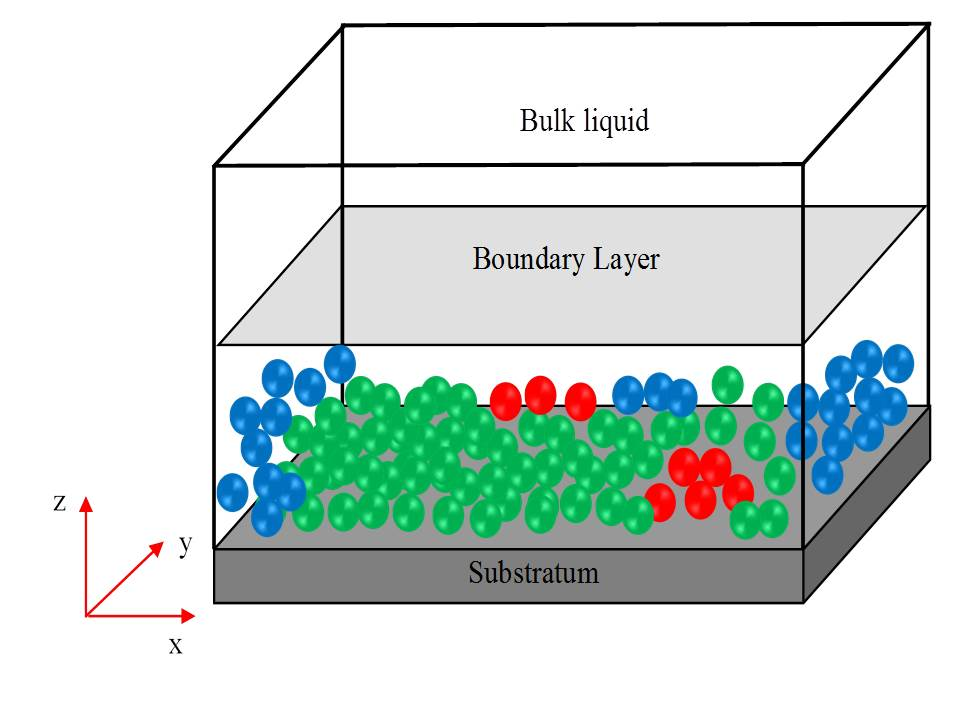
\includegraphics[width=.8\textwidth]{result2/box}
\caption[]{Computational domain for IB model of biofilms and floc}\label{box}
\end{figure}

%\subsection{Experimental design}
\subsection{Simulation data}\label{data2}
This section describes the procedure for generating the parameter combinations and variables at which the LAMMPS IB model is run. We run the IB model for a small sample of input parameters which are generated using a Latin Hypercube Design (LHD). This procedure provides data for training our emulator to approximate the major outputs. The LHD technique provides a good coverage of the input space with a relatively small number of design points. We use the "maximin" version of LHD technique that optimises samples by maximising the minimum distance between design points \citep{pd5}. Suppose we want to sample a function of $p$ variables: the range of each variable is divided into $n$ probable intervals, and $n$ sample points are then drawn such that a Latin Hypercube is created.

In this study, we generate an $n \times p$ variables Latin Hypercube sample matrix with values uniformly distributed on the interval [0,1]. We then transform the generated sample to the quantile of a uniform distribution. The parameters are varied within the range of $\pm100\%$ of the standard values given in Table \ref{mytab1} to cover a wide variation of the computer model outputs behaviour. 
We limit our analysis to just $n=300$ training points and ten replicates at each design point because of the expense of this computer model. The essence of repeated runs is to incorporate stochastic variations in our outputs. 

Let the design matrix which contains the input to the LAMMPS model be denoted by $\bX=(\theta^i_p, t, p=1,\ldots,27; i=1,\ldots,300)$, where the subscript $p=27$ represents 27 model parameters that are varied and 5 inlet concentration variables that represent the model initial conditions (see Table \ref{mytab1}), superscript $i$ denote the 300 different realisations (design points) and $t$ is the time slice in seconds at which the output data is recorded $t=1,\ldots,72$. The design matrix $\bX_{300 \times 32}$ denotes the input values at which the LAMMPS model is run for every combinations of $x_i$ which is a point in $\bX$, where $x_i$ represents $i^{th}$ row of $\bX$.  The simulator is run for about eight days (720000s simulation time). The output results are recorded at a time-step of 10000 seconds which gives about 72 different time slices.

 The simulator is run for both the floc and biofilms simulations. The following outputs are produced from the simulator particle diameter, mass, position (3-dimensional) and nutrient consumption at each time step. The time series output at each design point is denoted as a matrix $\bY=[\by_1,\ldots,\by_T]$, such that $\by=[y_1,\ldots,y_n]$,  where $T=72$ in this simulation and $n$ is the total number of particles at each time step. The number of particles $n$ at each time slice varies across the design points and, in particular, increasing with time as it expected for the microbes to be growing. %An additional independent simulation of 10 runs with ten replicates is performed for cross-validation purpose, but here, the simulation is run for a longer period than the previous simulations (~15 days simulation). 
%We consider emulation of floc which is summarised by aggregating all the individual microbe at each time step. 

\subsection{Outputs for emulation}\label{out1}
Figures (\ref{diag2}) show a spatially distributed nature of the the floc and biofilms making the emulation of these data a large dimensional problem. We preprocess the data by measuring the aggregated characteristic on them to reduce the dimensionality of the problem. Suppose at time step $t$, we summarize the individual particle at microscale (particle level) to a larger scale of biofilm/floc where we measure the following characteristics. 
\begin{itemize}
\item[(1)] Biofilms/floc total number of particles 
\item[(2)] Biofilms/floc particle composition  - calculate the proportion of each species, HET, AOB,NOB, EPS and DEAD
\item[(3)] Biofilms /floc total mass - $M_t =\sum \limits^n_{k=1} m_{kt}$, where $M_t$ is the total floc mass at time $t$ for all the species and $m_{kt}$'s are the individual particle level mass.
\item[(4)] Floc equivalent diameter/ biofilm height  -  There are two different ways to derive the floc equivalent diameter namely the volume and distance techniques. Under the distance approach, the diameter of the smallest circle that circumscribes the outer edge or sketch of the floc can be obtained by computing relative distances in $X-Y-Z$ positions of each of the particle from the center of mass of the floc aggregate. The sum of the maximum of this distances and radius of the particle with the largest distance will form the radius of the outer sphere as shown in Figure (\ref{diag2}). Suppose at time $t$, the distance in euclidean three-space between any two positions, say particle $p$ at position $P=(x_k,y_k,z_k)$ and floc center of mass at point $\tP=(x_0,y_0,z_0)$ is given as $d_{k}=\sqrt{(x_{kt}-x_0)^2+(y_{kt}-y_0)^2+(z_{kt}-z_0)^2}$, and $d_{t~eqv}=2(\max{(d_{k})}+r_{k'})$, where $r_{k'}$ is the radius of particle with largest distance and $x$, $y$ and $z$ are respective directions, $k=1,\ldots,n$. 
The second approach is to compute the total volume of the floc from the volume of each individual particle (each particle is taken as a sphere).
\begin{equation}
d_{t~eqv}=\sum^n_{k=1} \sqrt[3]{\frac{6V_{kt}}{\pi}}
\end{equation}
where $V_{kt}$ volume of individual spherical particle $k$ at time $t$, $\pi$ is a constant and $d_{eqv}$ is the floc equivalent diameter. The volume technique under-estimates the value of equivalent diameter.

\item[(5)] Biofilms/floc segregation index - The index measures the degree to which colocalized particles are genetically related to each other. Consider a particle $c_{ij}$ in a given a population of M particles such that $i=1,\ldots,M$, and identify related particles within a distance of 10 diameter length with the same phenotype as  $c_{ij}$, see further details in \citet{co9}.
The index is given as $\sigma_t=\frac{1}{M}\sum \limits_{i=1}^M \Big(\frac{1}{N}\sum \limits_{j=1}^N\rho(c_i,c_j)\Big)$, where
\begin{align}
\rho(c_i,c_j)=\begin{cases}
 0, \text{$c_j$ is not the same phenotype as $c_i$}\\
1, \text{$c_j$ is the same phenotype as $c_i$} 
\end{cases}
\end{align}
\item[(6)] Biofilm/floc fractal dimension - Fractals are of rough or fragmented geometric shape that can be subdivided in parts. 
Fractal dimension of a biofilm or floc is a measure of the complexity of its external shape \citep{co7}. It reflects the hydrodynamic environment that produces microbial aggregates. The fractal dimension can also be used to study the process of aggregation in wastewater treatment where the characteristics of the aggregates play a crucial role in the performance, and operational stability \citet{co6}. Unlike \citet{co7} that uses the relationship between the object area and perimeter to calculate the fractal dimension, we used the ratio of radius of agglomerates to the mean radius of the particles as given by the formula below. 
\begin{equation}
F_{Dt}=\frac{log(R_a/R_m}{log(n)}
\end{equation} 
where $F_{Dt}$ is a fractal dimension, $R_a=\sqrt \frac{\sum \limits_{k=1}^n m_{kt} d_{kt}^2}{\sum \limits_{k=1}^n m_{kt}}$ and 
$R_m=\frac{\sum \limits_{k=1}^n r_{kt}}{n}$, $d_{kt}$, $r_{kt}$ and $m_k$ are the particle diameter, radius and mass respectively. 
The parameter $\delta$ is a measure of active layer thickness of the floc and/or biofilms and is given as the ratio between the nutrient transport to the biomass and the nutrient consumption by the bacteria. In addition, $\delta$ determines the resulting shape of the floc to a certain extent, large $\delta$ values signify a large nutrient availability for the growing floc/biofilms thus decreases the heterogeneity within the floc and smooth surface floc or biofilm is formed as in Figure \ref{diag2}(a) while a low $\delta$ value gives a more irregularly shaped (fractal) floc is formed in Figure \ref{diag2}(b).

\item[(7)] Simpson diversity index - a measure of diversity of a biofilm/floc, $D_t=1-\frac{\sum n(n-1)}{N(N-1)}$ where $n$ is the total number of organisms of a particular species and $N$ is the total number of organisms of all species. 

\item[(8)] Biofilm surface roughness - 

\end{itemize}

\begin{figure}[!ht]
%\centering
\begin{subfigure}[b]{.5\textwidth}
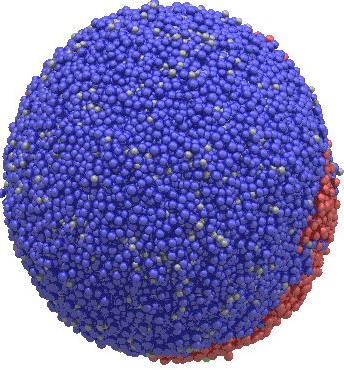
\includegraphics[width=.8\textwidth]{result2/diag1b}
\caption{$\lim_{\delta \to \infty}$}
\end{subfigure}\hspace*{-1.5em}
\centering
\begin{subfigure}[b]{.5\textwidth}
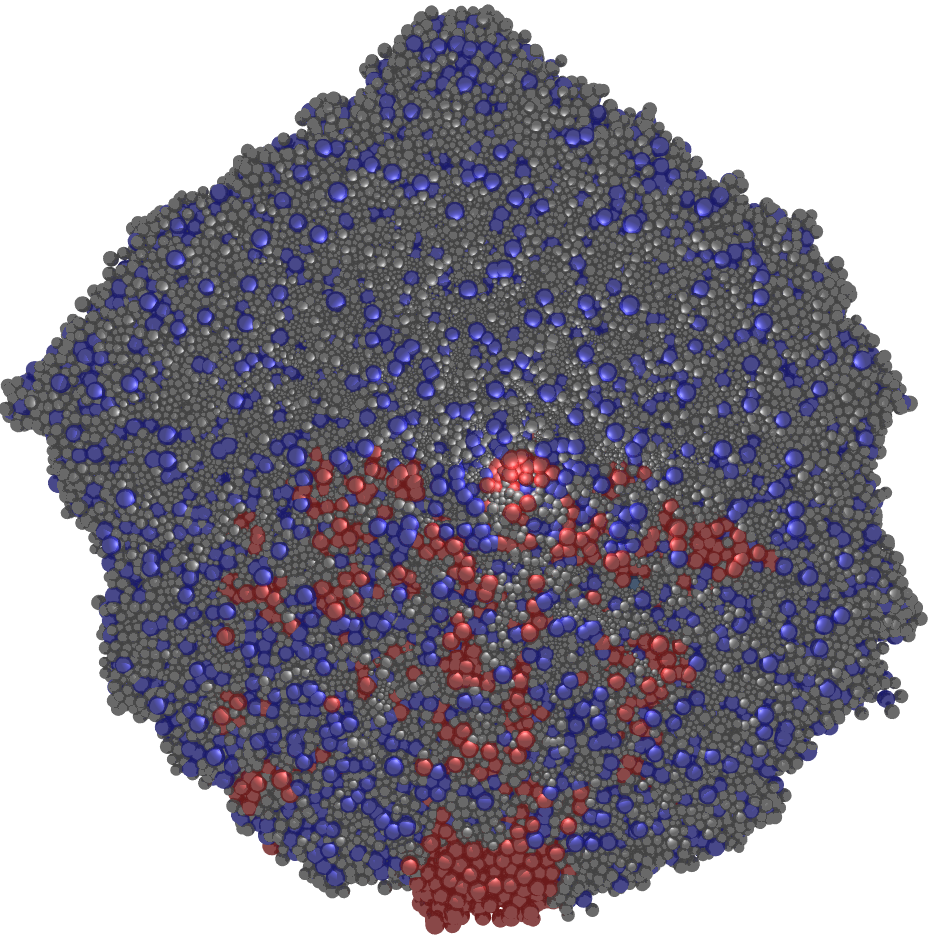
\includegraphics[width=.8\textwidth]{result2/plot366}%{result2/diag1bb}
\caption{$\lim_{\delta \to 0}$}
\end{subfigure}\vspace*{-1.5em}

\begin{subfigure}[b]{.5\textwidth}
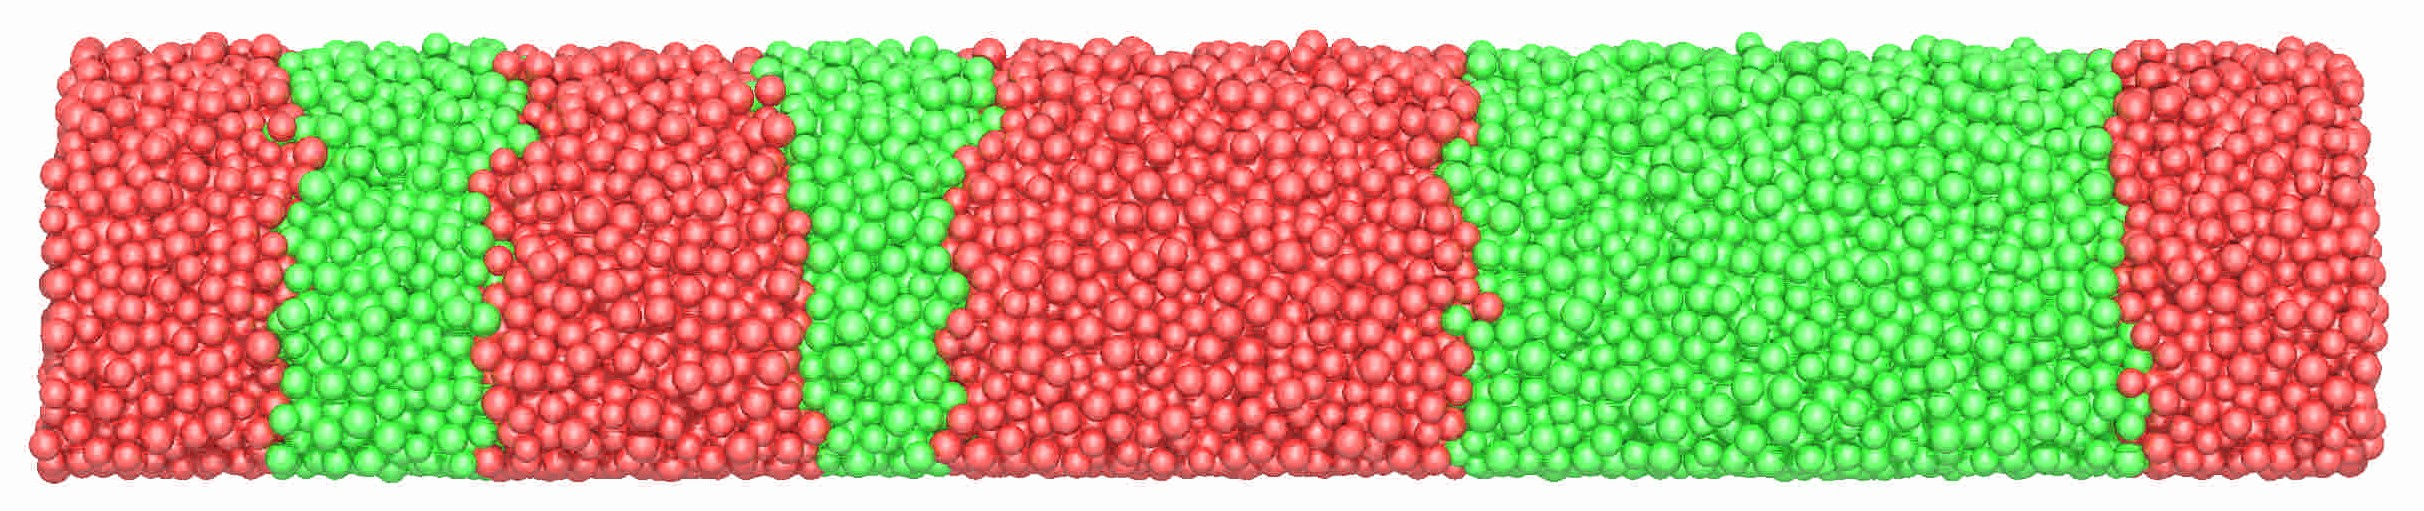
\includegraphics[width=.8\textwidth]{result2/bio11}
\caption{$\lim_{\delta \to \infty}$}
\end{subfigure}\hspace*{-1.5em}
\centering
\begin{subfigure}[b]{.50\textwidth}
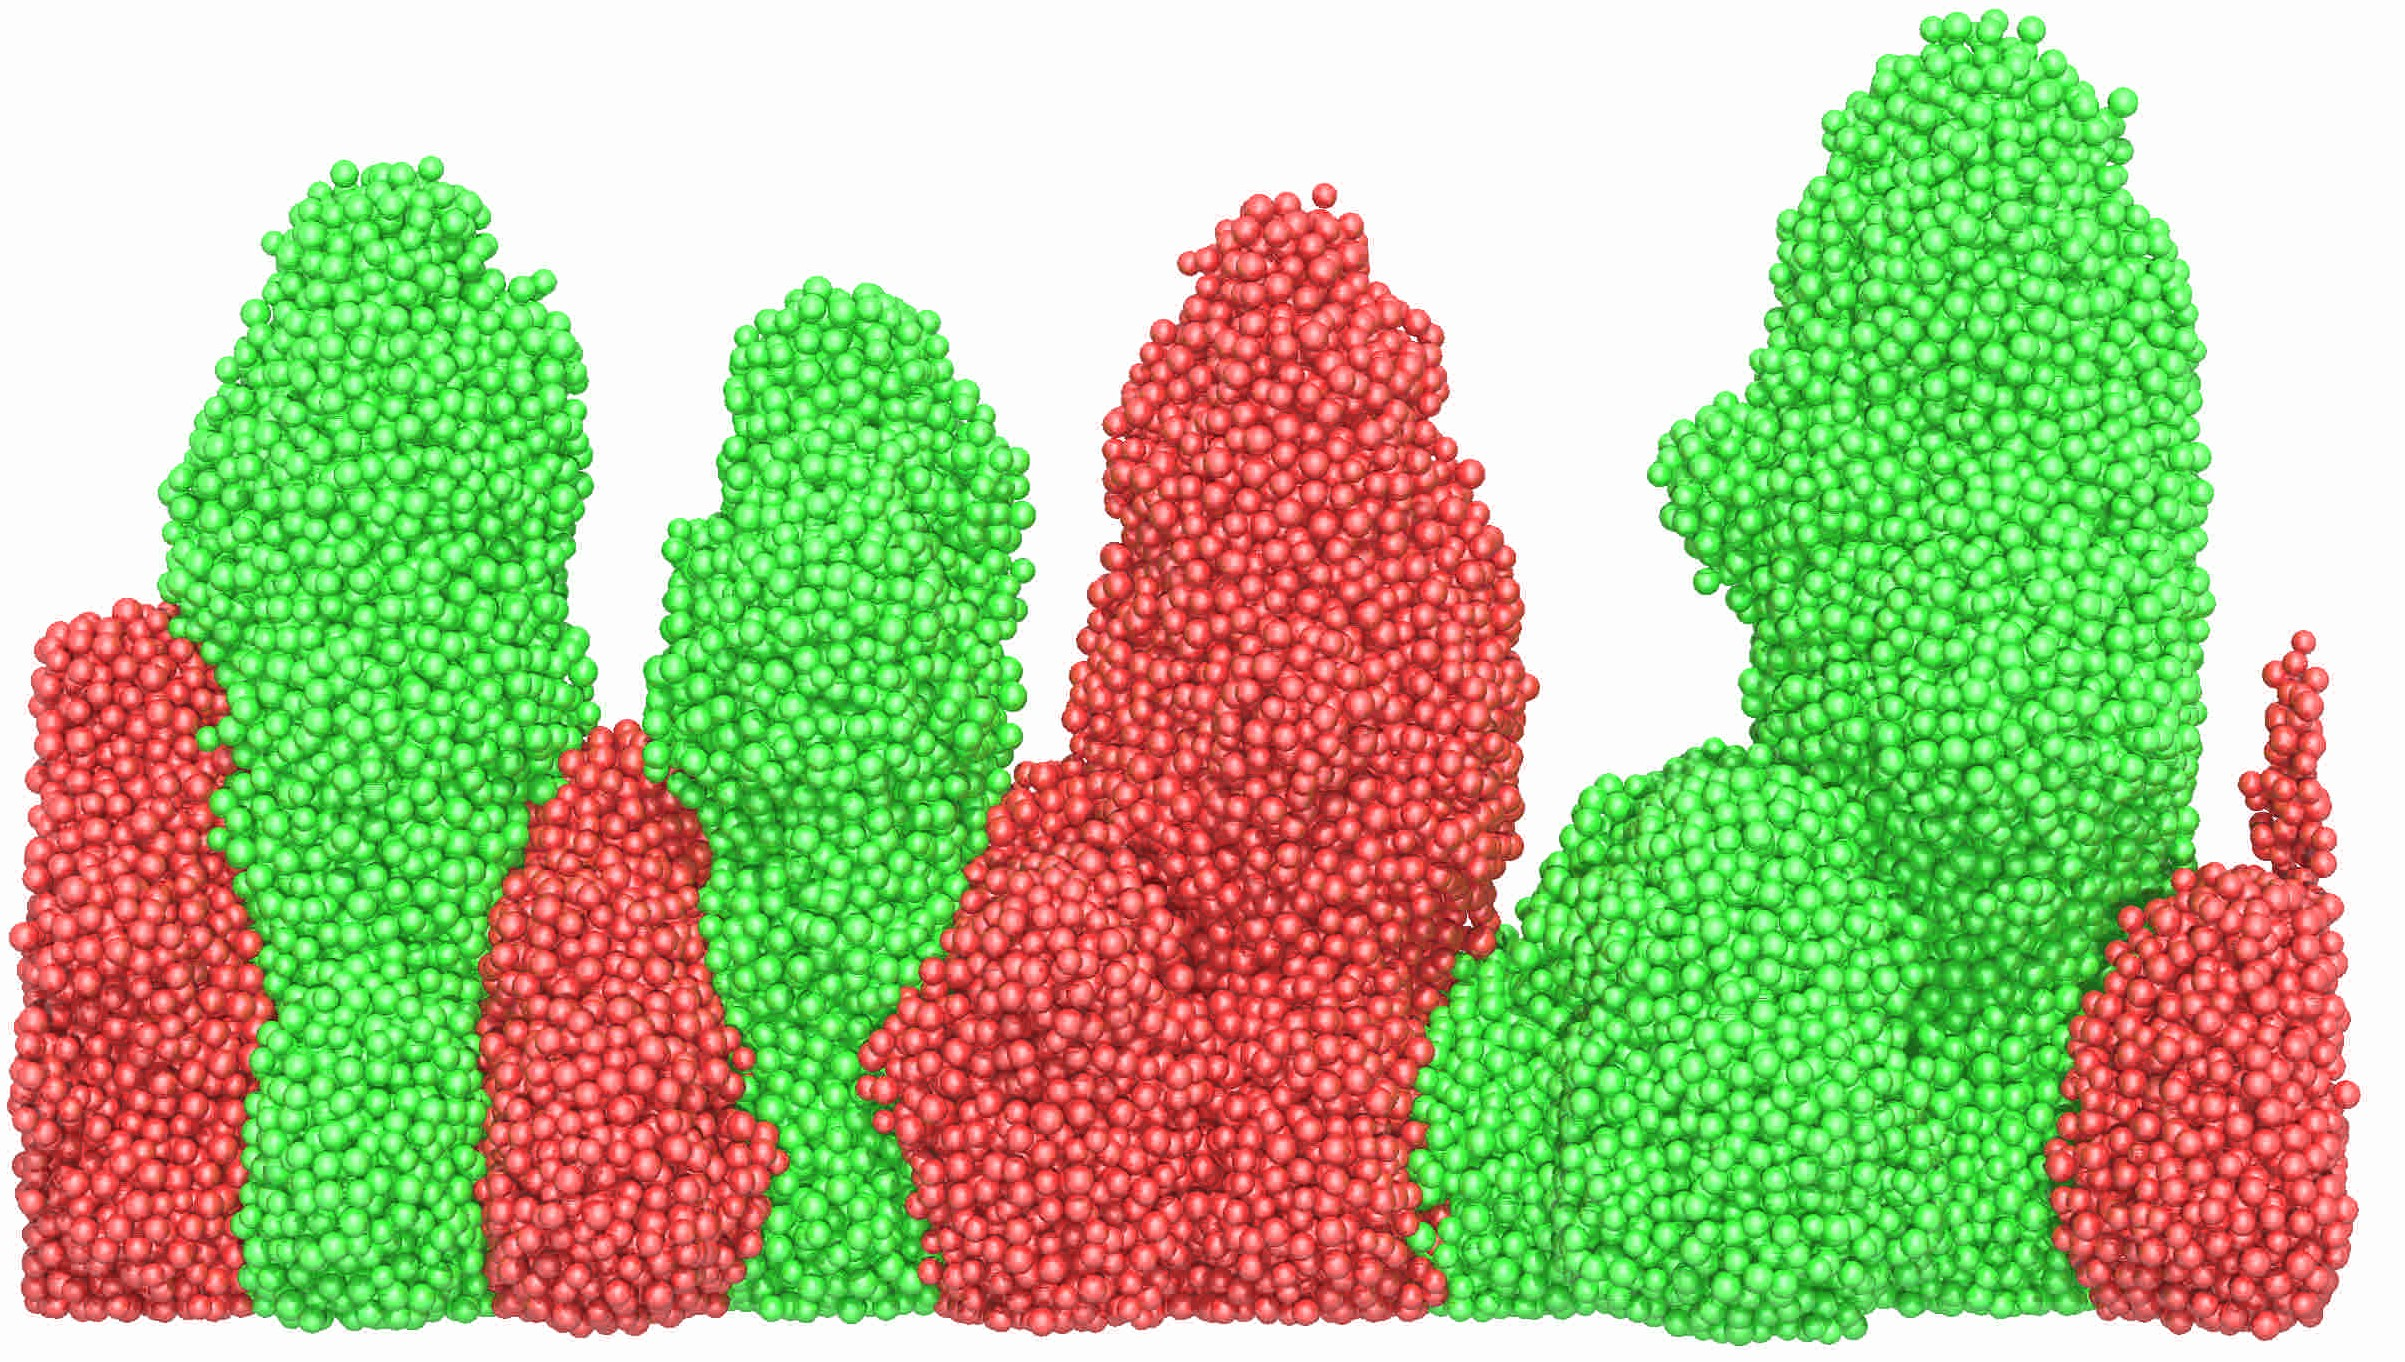
\includegraphics[width=.8\textwidth]{result2/bio22}%{result2/diag1bb}
\caption{$\lim_{\delta \to 0}$}
\end{subfigure}\vspace*{-.5em}
\caption{Transformation of microscale particles to floc at the mesoscale for a particular time. Floc equivalent diameter is the diameter of the smallest sphere that circumscribes the outline of the projected floc. $\delta=\sqrt \frac{S_{bulk} D Y_s}{\mu_{max}\rho L^2}$, $S_{bulk}$,D,$Y_s$, $\mu_{max}$ ,$\rho$ and $L$ are the bulk nutrient concentration, diffusion coefficient, yield
coefficient, maximum specific growth rate, biomass density, and boundary layer thickness respectively. The top-left - smooth floc: top-right - rough floc: bottom-left - smooth biofilms: bottom-right - rough biofilms.}\label{diag2}
\end{figure}

\begin{figure}[!ht]
\begin{subfigure}[b]{.5\textwidth}
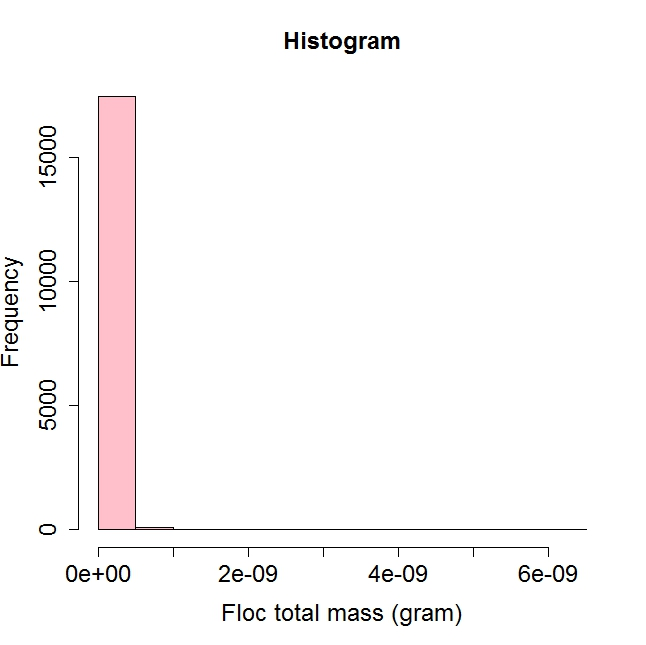
\includegraphics[width=.8\textwidth]{p2/hist_mass}
%\caption{$\lim_{\delta \to \infty}$}
\end{subfigure}\hspace*{-1.5em}
\centering
\begin{subfigure}[b]{.50\textwidth}
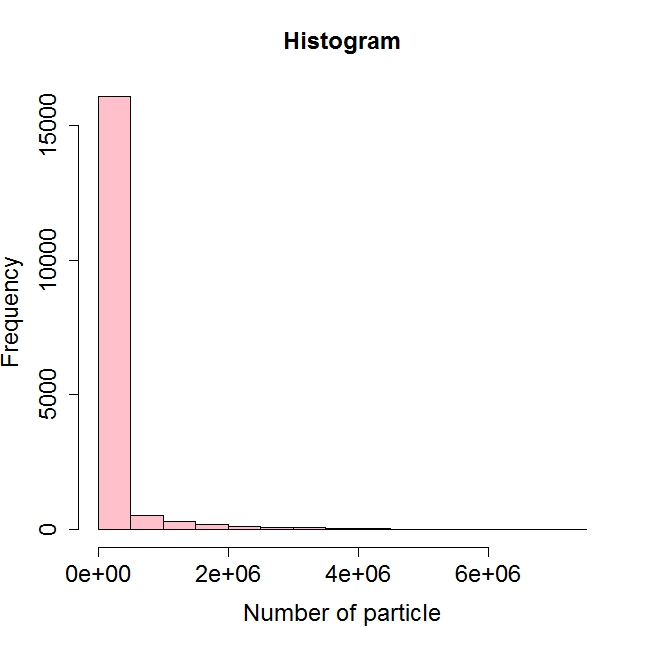
\includegraphics[width=.8\textwidth]{p2/hist_nop}
%\caption{$\lim_{\delta \to 0}$}
\end{subfigure}\vspace*{-.5em}
\caption[]{Histogram of floc total mass and particle growth showing a large variation in these datasets}
\end{figure}\label{hist}


\begin{figure}[!ht] 
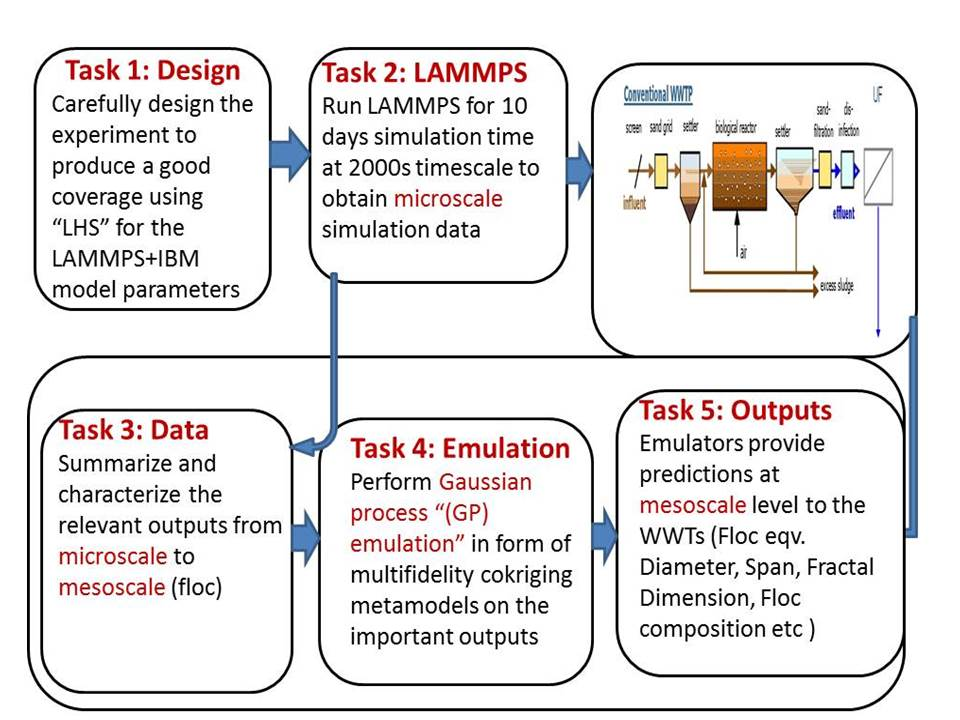
\includegraphics[width=1\textwidth]{result2/box2}
\caption[]{Schematic diagram showing key emulation stages}\label{diag2c}
\end{figure}

\newpage
\section{Methods}
 A Bayesian framework for emulation is almost always based on the assumption that a Gaussian process prior distribution can be specified for unknown parameters and hyperparameters.  Under a Bayesian perspective, unknown parameters are treated as random variables. The given prior distribution can be updated from training data, and a posterior distribution can be obtained. The posterior distribution is also a Gaussian process.
A popular method for constructing a metamodel is the Gaussian process regression also called kriging. 
 A major difficulty with GP modelling is the computational effort associated with dealing with huge amount of data, as computer time scales are of order $O(n^3)$ where $n$ is the number of observations. Several techniques have been adopted to overcome this computational problem. Earlier techniques are documented in \citet{q10} and \cite{q47}. GP emulation is based on the Bayesian technique and experimental design of computer experiments for predicting model outputs at test input point \citet{q7} and \citet{70}. A GP emulator assumes that a simulator output is an unknown function $g(.)$ with a  given prior distribution for $g(.)$, using the Bayesian approach and update this distribution with some data obtained from the simulator runs. We are implementing GP technique in the form of cokriging because of its wide applicability and flexibility. %Another additional benefit of GP modelling is the quantification of the model uncertainty.


\subsection{Cokriging}\label{cokk}
We use cokriging which is a multivariate extension of kriging to $m$ observation types. Cokriging has been widely applied in a various area especially in multifidelity surrogate models where there are an array of $m$ levels of code usually from the expensive (accurate) to the less expensive (crude) simulators which are modelled jointly. It involves emulation of a function that is costly to evaluate which is enhanced by data from a cheaper simulation of the function \citep{co3,co5}.  In this paper, we are assuming that the characterised outputs from the IB models have $m$ code levels. We shall briefly describe what the kriging technique entails providing a basis for the theory of cokriging.

Kriging is a geostatistical technique for interpolating the value of an unknown random observation from data $\by(\bx)$ observed at known locations. Kriging models are also commonly used for building cheaper surrogate model of expensive computer codes \cite{pd1,pd2, pd3,pd6}. The two stage techniques describes in \citet{pd11} are combined as a single step., where a given scalar output $\by(\bx)$ can be decomposed into a mixture of deterministic (non-random trend) and a residual random variation. The trend could be modelled as a constant in ordinary/simple kriging or as an $n^{th}$ order polynomial in universal kriging. We discuss the universal kriging technique that we use in this paper. The model formulation is given as
\begin{equation}\label{geneq2}
\by(\bx)= f(\bx) + \boldsymbol \varepsilon(\bx)
\end{equation}
where $\by(\bx)$ is the output of interest (say, floc equivalent diameter). The deterministic function $f(\bx)$ is the mean approximation of the expensive computer simulator (eg IB models) and $f$ is a polynomial function. Under this assumption, $f(x)$ can be modelled as
\begin{equation}
f(\bx) = \sum_{j=1}^{p} \beta_j h_j(x) =\bH(x) \bbeta
\end{equation}
$\bbeta=[\beta_1,\ldots,\beta_p]$ is a $(p\times 1)$ vector of unknown regression coefficients and $\bH(x) = \Big[h_1(x), . . . , h_p(x)\Big]^T$ is a $(n\times p)$ matrix of regression functions,
$\varepsilon(\bx)$ is a stochastic Gaussian process with mean zero and characterize by its covariance function
$K=Cov(\varepsilon(\bx),\varepsilon(\bx)) = \sigma^2\bC(\bx,\bx')$, where $\sigma^2$ denotes the variance of $\varepsilon(\bx)$ also called process variance and $\bC$ is a $(n\times n)$ positive definite matrix of correlation between $\varepsilon(\bx)$'s at the experimental design points. We are assuming a univariate output and a deterministic computer model.

Similarly, $\bt(x^{new}) = \Big[Cor(x_1, x^{new}), \ldots,Cor(x_n, x^{new})\Big]^T$ for the $(n\times 1)$ vector of correlations between the $\varepsilon(\bx)$'s at the design points and new input points $x^{new}$. We use an exponential correlation function $\bC=\Big \{\exp(-(x-x')^T \boldsymbol \alpha (x-x')) \Big\}$, where $\boldsymbol \alpha$ is the correlation hyperparameters to be estimated from the data \citet{pd4,pd18,pd19}.
The best linear unbiased predictor for universal kriging model is given as
\begin{equation}\label{man}
\mu^{\bullet}_{uk}(x) = h^T(x)\hbbeta+ \bt^T(x)\bC^{-1}(\by -\bH\hbbeta)
\end{equation}
and variance
\begin{multline}\label{olu2b}%\tag{A.9}\label{olu2}
\begin{split}
\bK^{\bullet}_{uk}=\hat \sigma^2 \Big \{C(\bx,\bx') -\bt(\bx)^T\bC^{-1} \bt(\bx) + \\ \Big ( h(\bx)^T-\bt(\bx)^T\bC^{-1}\bt(\bx) \Big )
(\bH^T\bC^{-1}\bH)^{-1}\Big (h(\bx')^T-\bt(\bx')^T\bC^{-1}\bt(\bx') \Big )^T
\Big \}.
\end{split}
\end{multline}
See more details in \citep{pd4,pd5,pd20}.
Suppose we now have $m$ output levels of code $\bY(x)=(Y_1(x), \ldots, Y_m(x))$, %$x \elem R$
The $k^{th}$ output $y_k(x)$ is modelled as a Gaussian process $y_k(x) = Y_k(x)$. We use an autoregressive ($AR$) model earlier proposed by \citet{co4} which is based on Markov property such that $Cov(Y_t(x), Y_{t-1}(x′)|Y_{t-1}(x)) = 0, x \neq x'$
and recently applied by \citet{co1}. The model formulation assumes
\begin{equation}\label{cok1}
Y_k(x) =\rho_{k-1}Y_{k-1}(x) + \delta_k(x)
\end{equation}
for $k\in (2,\ldots,m)$, where $\delta_k(x)$ is a Gaussian process that models the bias between the output $k$ and the output $k-1$ adjusted and $\rho_{k-1}$ is the scaling factor between $Y_k$ and $Y_{k-1}$. The $\rho_{k-1}$ can be further treated as a linear regression function such that 
\begin{equation}
\rho_{k-1}(x) = g^T_{k-1}(x)\gamma_{k-1}
\end{equation}
and $g^T_{k-1}(x)$ is a vector of regression functions with covariance function of the form
$c_k(x, x′) = \sigma^2_k r_k(x - x′; \balpha_k),$
 where $\sigma^2_k$ is the variance of the Gaussian process and $\balpha_k$ are the correlation hyper parameters of correlation function $r_k$. 
In addition, since each of $Y_k(x)$ is a GP then the joint process ($Y_1(x), \ldots, Y_m(x)$) is a multivariate GP with mean
\begin{equation}
E[Y_k(x)|\sigma^2, \balpha, \bbeta, \gamma] = h′_k(x)^T \bbeta
\end{equation}
and covariance function
\begin{equation}
cov \Big[Y_k(x),Y_k(x')|\sigma^2, \balpha, \bB, \gamma_k \Big]=\sum_{k=1}^m \sigma^2_k \Big( \prod \limits_{i=k}^{k-1} \rho^2_i(x)\Big) r_k (x-x′;\balpha_k),
\end{equation}
where $\sigma^2=(\sigma_1^2,\ldots,\sigma_k^2)$, $\balpha=(\balpha_1,\ldots,\balpha_k)$,  $\bB=(\bbeta_1,\ldots,\bbeta_k)$ and $\gamma=(\gamma_2,\ldots,\gamma_k)$,  
$$h'_k(x)^T=\Bigg( \Big( \prod \limits_{i=1}^{k-1} \rho_i(x)\Big) g^T_1(x), \Big( \prod \limits_{i=2}^{k-1} \rho_i(x)\Big) g^T_2(x), \ldots,\rho_{k-1} g^T_{k-1}(x),g^T_k(x) \Bigg),$$ $\bX_k$ is a design matrix and
$\Psi_k(\bX_k, \bX_{k'})$ is a $(n_k \times n_{k'})$ correlation matrix.
Unlike \citet{co1} and \citet{co2} that uses the Bayesian estimation technique, in this paper we follow a likelihood maximization approach of \citet{co3} and in order to simplify our approach, we assume $k=2$ so that equation \ref{cok1} can be rewritten as 
\begin{equation}
Y_2(x) =\rho Y_{1}(x) + \delta(x)
\end{equation}
where the design matrix is now re-defined as
\begin{equation}
\bX=\Big(\bX_1, \bX_2    \Big)^T=(\bx^{(1)}_1,\ldots,\bx^{(n_1)}_1,\bx^{(1)}_2,\ldots,\bx^{(n_2)}_2)^T
\end{equation}
such that
\begin{equation}
\bY=\Big(\bY_1(\bX_1), \bY_2(\bX_2)  \Big)^T=(Y_1(\bx_1^{(1)}),\ldots,Y_1(\bx_1^{(n_1)}),Y_1(\bx_2^{(1)}),\ldots,Y_1(\bx_2^{(n_2)}))^T.
\end{equation}
The conditional distribution of the output at a new target point $\bx^{new}$ under a universal cokriging formulation is given as
\begin{equation}
\Big[\by_2(\bx^{new})|\by=\by_1,(\bbeta_1,\bbeta_2,\rho),(\sigma_1^2,\sigma_2^2),(\balpha_1,\balpha_2)\Big] \sim N(\mu_{Y_2}(\bx^{new}),\bK(\bx^{new}))
\end{equation}
the mean and variance functions are given respectively as
\begin{equation}\label{cokmean}
\widehat\bmu_{\by_2}{(\bx)}= h^T(\bx)\hbB+ \bt^T(\bx)\bSigma^{-1}(\by -\bH\hbB)
\end{equation}
\begin{equation}\label{cokvar}
\widehat \bK_{\by_2}(\bx)=\hat\rho^2\hat \sigma_1^2+ \hat\sigma_r^2 - \bt^T(\bx)\bSigma^{-1}\bt(\bx),
\end{equation}
where 
\[ 
\bB=
\left(\begin{array}{cc}
\bbeta_1\\
\bbeta_2
\end{array} \right)
\quad \mbox{,}
\quad 
\by=
\begin{pmatrix}
y_1\\
y_2
\end{pmatrix}, 
\quad
h'=(\rho g_1^T(\bx),g_2^T(\bx)),
\]
\begin{equation}
t(\bx)=\rho \sigma_1^2 \Psi_1(\bx,\bX_1), \rho^2\sigma_1^2\Psi_1(\bx,\bX_2)+\sigma_r^2\Psi_r(\bx,\bX_2))^T,
\end{equation}
and covariance matrix given as
\[ \bSigma=
\left(\begin{array}{cc}\label{cokcovv}
\sigma_{1}^2\Psi_1(\bX_1,\bX_1)   ~~~~~~~~~~~~~~~~~~~~ ~~ \rho\sigma_{1}^2\Psi_1(\bX_1,\bX_2)\\
\rho\sigma_{1}^2\Psi_1(\bX_2,\bX_1)  ~~~~~~ \Big(\rho^2\sigma_{1}^2\Psi_1(\bX_2,\bX_2) + \sigma_{r}^2\Psi_r(\bX_2,\bX_2)\Big)
\end{array} \right)\]

\[ \bH=
\left(
\begin{array}{cc}
g_1^T(x_1^{(1)}) ~~~~~~~~0\\
\vdots   ~~~~~~~~~~~~~~~~~~ \vdots       \\
g_1^T(x_{n_1}^{(1)}) ~~~~~~~~0  \\

\rho g_1^T(x_1^{(2)}) ~~~~~~~~g_2^T(x_1^{(2)})\\
\vdots   ~~~~~~~~~~~~~~~~~~ \vdots       \\
\rho g_1^T(x_{n_2}^{(2)}) ~~~~~~~~g_2^T(x_{n_2}^{(2)})
\end{array} 
\right)
 \quad = \quad
\begin{pmatrix}
F_1(\bX_1)~~~~~~~~~~0\\
\rho F_1(\bX_2) ~~~~~~~F_2(\bX_2)
\end{pmatrix}.
\]
The next problem is how to estimate the unknown parameters $(\bbeta_1,\bbeta_r,\rho,\sigma_1^2,\sigma_r^2,\balpha_1,\balpha_r)$ and incorporate stochasticity in our model formulation which we describe in the Appendix 3. 
%\item \alert{Univariate} - incorporate nugget terms in the form of empirical variance derived from replicates
%\item The extension for noisy observations, covariance $K=\sigma^2\bC$ is replaced by \alert{$ \sigma^2\bC+diag(\btau^2_1,\ldots,\btau^2_n)$}, where $\btau^2=\tau^2_1,\ldots,\tau^2_n$ are the noise variances
%\newline
%\item  \alert{Multivariate} - Follow  Kleijnen \& Beers(2005) approach of emulating a scale response
%\newline
%\item The scale response is derived by repeating the simulation $k$ times at each design point such that
%$\by'=\frac{\bar \by-\hat  f}{\mathbf{\sigma}^2/\sqrt{k}}$, where $\bar \by(x_i)=\frac{\sum \limits_{j=1}^k\by_{ij}}{k}$, $\sigma^2(x_i)=\frac{\sum \limits_{j=1}^{k}(\by_{ij}-\bar \by)^2}{k-1}$ and $\hat  f$ is estimate of main signal function
%\newline
%\item Apply kriging model to $\bY=[\by'_1,\ldots,\by'_m]$

%A Gaussian process model could not be applied directly to the stage 1 because of the computational difficulty in the sample size coupled with a significant number of parameters to be estimated. GP scales cubically with the number of observations $O(N^3)$, which is not appropriate for our present data, even after averaging decadally and sampling from each scenario. The data matrix contains over 4.5 million observations. Using GP for residual interpolation is possible. However, this approach still has a high computational cost, and it is necessary to reduce the spatial resolution and aggregate data to a country level to reduce the computational load. Our procedure is described below. 

%\subsection{Emulation procedure}
\section{Procedure for emulating IB model outputs}
Our emulation can be categorised into two broad groups. Emulation of the floc and biofilms. There are two different approaches to each of the problem. Firstly, we could emulate the individual particle at the micro levels and use the emulator to link the simulator output at a mesoscale level for as a floc or biofilm. This approach is currently not practicable owing to a large number of simulation data involves, although it could be possible to perform some forms of data reduction. It is likely that pattern decomposition might even complicate our problem. 

The second approach that we adopt in this study is to focus on the cluster of particles as flocs and biofilms because of a vast number of data involve and emulate their interested properties described in subsection \ref{out1}. A single run of LAMMPS model consists of a simulation over many time steps which requires much computer workload and time taken. Here, we shall focus on the floc emulation and in particular we shall describe the emulation of Simpson species diversity, total mass, the number of particles, fractal dimension and equivalent diameter of the floc to simplify our approach. Emulation of other outputs will follow a similar procedure. The floc is treated as a ball of a sphere, and we estimate the diameter of a sphere that circumscribes its boundary/outline. The center of the sphere will be equivalent to the center of mass of the component particles as shown in Figure (\ref{diag2}). The detailed procedure of emulating the floc parameters will be described in this section and for the biofilm is deferred to next section. 

Some of the challenges of LAMMPS emulation are the nature of the outputs produced from the model which make it much difficult to emulate. The LAMMPS model is expensive to evaluate, i.e., slow and difficult to run for a large parameter space of interest, which limits the amount of information available for emulation. The model is stochastic in nature; this introduces much randomness in the data. The model is also dynamic because the data are arranged as a sequence of outputs at different time points. Finally, the model produces high-dimensional and multiple outputs which make the emulation more computationally demanding than usual.

Despite all these caveats, the good news is that there is a large knowledge base addressing these problems. The stochasticity in the model is handled by performing multiple runs and average the key outputs which are then taken as deterministic in nature. Secondly, we fit a heterogeneous cokriging model that incorporate noise in the form of empirical variance derived from the repeated simulation data.

\subsection{Dynamic emulation}
Due to the dynamic nature of output data from LAMMPS model, we apply a novel dynamic emulation strategy within a cokriging framework. Dynamic emulation models the evolution or trajectory of random variables over some time-steps. Emulation of time-series data or physical processes that evolve with time which implies that model output at time $t$ becomes an input to the model at time $t+1$. The model can be written as 
\begin{equation}\label{dyna3}
\by_t = f(\bx_t, \by_{t-1}),
\end{equation}
where $\by_{t-1}$ is the state vector at the previous time step for $t={1,\ldots,T}$, and $\bx_t$ (each $\bx_t$ corresponds to design matrix $X_{300 \times 32}$) are the inputs at time $t$ which includes the model parameters, forcing and initial conditions (see Table \ref{mytab1}). We use a single-step emulation technique proposed in \citet{pd12}. Under the single-step procedure, the method assumes that a simpler, single step emulator can be built from a dynamic computer model, and the resulting emulator can be used repeatedly to generate the full-time series of the predictions up to the number of desired time points. This framework reduces the dimension of the problem and enables us to capture the complete behaviour of characterised outputs over a number of time steps.

%Firstly, under the multi-step emulation procedure, we can emulate a complete multi-step run of the computer model. One of the ways to proceed with this according to \citet{pd14} is to treat the problem as a multivariate output simulator and develop a multi-output emulator where the dimension of the output space is given as $T$. Closely related to this approach, is to build one single-output emulator that incorporates time as an additional input to the emulator such that $\by_t = f(\bx,t)$, where the training data for building emulator consists $nT$ data points. The limitation of this approach is that it is inefficient in practice because the dimension of the data becomes vast which introduces additional computational difficulty. The third variant is to emulate each time step, which produces an emulator that is specific to a particular time step, an approach that assumes independence between the time steps. This method was used in \citet{pd27} but is not suitable for our present data. Here, where are interested in the temporal correlations across the time steps, and specifically for using an emulator to scale up LAMMPS model outputs from an order of O($10^6$) particles to O($10^{13}$) particles, i.e., for making multiple-step ahead predictions. 

\subsubsection{Single-step emulation}
We follow a similar procedure described in \citet{pd12} and \citet{pd15}. Starting from initial run of the model at time $t_0$, we construct the single step emulator $\by_1 = f(\bx_1, \by_{0})$ using a GP regression in form of cokriging on the five chosen outputs. One of the usefulness of dynamic emulation is to make a multiple step ahead predictions using iterative technique to repeat one-step-ahead predictions until the desired number of points. We proceed sequentially, feeding back the entire output distribution from the cokriging model, such that at time step $t=1$, and for input $(\bx_1,\by_0)$, we sample from the distribution of $f(\by_0,\bx_1)$, the model output is given as $\tby^{(s)}_1 \sim N \Big(\mu^{\bullet}(\bx_1,\by_0), \bK^{\bullet}(\bx_1,\by_0)\Big).$
For the next prediction at time $t=2$, the input data $\bx_2$ is augmented by complete distribution $\by^{(s)}_1$ such that $\bX_2=[(\bx_2,\tby_1)]^T$,  then we generate sample from the distribution of $f(\tby^{(s)}_1,\bx_2)$ and denote as $\tby^{(s)}_2 $.%, note that distribution of $\tby^{(s)}_2 $ is no longer normally distributed.
%then we have $$\tby^{(s)}_2 \sim N \Big(\mu^{\bullet}(x_2,\tby^{(s)}_1), \bK^{\bullet}(x_2,\tby^{(s)}_1)\Big).$$
This procedure is repeated until $T-1$ steps is reached. The construction of single-step emulator is summarized below:
\begin{itemize}
 \item[{(i)}] Sample 280 points randomly from original 300 points and formulate a single step emulator using equation (\ref{dyna3}) such that $\by_1=f(\bx,\by_0)$, where $\bx$ is the new design matrix for running the LAMMPS model for the single step function, $\bx$, as usual, include initial conditions and calibrated (constant) parameters while the corresponding output is the value of current state variable $\by_t$.

\item[{(ii)}] Perform cokriging as described in subsection \ref{cokk}, where we use linear mean and exponential covariance functions. The parameters $\hat\theta=(\bbeta_1,\bbeta_r,\rho,\sigma_1^2,\sigma_r^2,\balpha_1,\balpha_r)$ are estimated by MLE technique.

\item[{(iii)}] Compute the posterior distribution of $\Big(f(.)|\by,\hat\theta \Big)\sim N \Big(\mu^{\bullet}(x_0), \bK^{\bullet}(x_0)\Big)$ where $\mu_{y2}^{\bullet}(x)$ and $\bK_{y2}^{\bullet}(x)$ are the cokriging predictor and variance defined in equations (\ref{cokmean}, \ref{cokvar}) respectively.

\item[{(iv)}] Use the emulator to simulate from $\Big(f(.)|\by_1,\hat\theta\Big)$  to obtain $\tby^{(s)}_{1}$ and then iterate the next steps for $t=1,\ldots,T-1$ to give a full time series $\Big[\tby^{(s)}_1,\ldots,\tby^{(s)}_{T-1}\Big]$. 

%\item[{(v)}] Derive a new training data by augmenting the original data with simulated time series and rebuild the single-step emulator with the new training data given below. 
%\[ 
%\left( \begin{array}{ccc}
%\mbox{Original inputs}\\
%~\vdots \\
%(\by_0,\bx_1)\\
%(\tby_1,\bx_2)\\
%~~\vdots \\
%(\tby_{T-1},\bx_T) \end{array} \right)
% = 
%\left( \begin{array}{ccc}
%\mbox{Original outputs}\\
%~\vdots \\
%\tby^{(s)}_1\\
%\tby^{(s)}_2 \\
%~\vdots \\
%\tby^{(s)}_{T}\end{array} \right).
%\] 
%\item[{(vi)}] Simulate $\tby^{(s)}_{t+1}$ from conditional distribution $\Big(f(.)|\by_t,\hat\theta\Big)$.  
%\item[{(vi)}] Repeat the entire process many times to obtain $\tbY^{N}=\Big[\tby^{(s)}_1,\ldots,\tby^{(s)}_{T-1}\Big]^N$, for $s=1,\ldots,N$, where $N$ is the number of Monte Carlo sample.
\end{itemize}
%Here, we summarize the approximation technique according to \citet{pd12}. This new procedue is based on the assumption that augmentation of training data at each iteration step will have a relatively minimal effect provided that we use a large sample size for building our single-step emulator, in other words, additional data at each step could be discarded. In addition, since our training data for the single step emulator $\by_t = f(\bx,t)$ is modelled as a GP, thus makes it difficult to derive a joint distribution for $\by_1,\ldots,\by_T$ in a closed form, rather a normal approximation is proposed to estimate the marginal distribution of each $\by_t$ for $t=1,\ldots,T$. Suppose, the marginal distribution of $\by_t$ can be approximated as $\by_t \sim N\Big(\mu_t(.), \bK_t(.)\Big)$, where $\mu_1 =\mu^{\bullet}(x_1,y_0)$ and $\bK_1=\bK^{\bullet}\Big((x_1,y_0),(x_1,y_0)\Big)$, $\mu^{\bullet}(.)$ and $\bK^{\bullet}(.,.)$ are already defined in equations (\ref{man} and \ref{olu2b}) respecctively.

%Then we have
%\begin{equation}
%\mu_{t+1}=E\Big(\mu^{\bullet}(\by_t, x_{t+1})|f(\by)\Big),
%\end{equation}
%\begin{equation}
%\bK_{t+1}=E\Big(\bK^{\bullet}(x_{t+1},\by_t),(x_{t+1},\by_t)|f(\by)\Big) +var \Big(\mu^{\bullet}(\by_t, x_{t+1})|f(\by)\Big).
%\end{equation}
\subsubsection{Normal approximations}
One of the limitations of the single-step emulation procedure is that it is highly prone to numerical problems associated with ill-conditioned covariance matrix as training data is augmented. Moreover, an additional computational cost is often involved. \citet{pd12} proposed a simple normal approximation to the above procedure that we applied in this study. This approach is comparable to \citet{pd17} technique applied on a nonlinear dynamic systems to propagate uncertainty in an iterative multiple-step-ahead predictions. Now, we can estimate the two quantities in equations \ref{cokmean} and \ref{cokvar} in Appendix 3 using simulation from Monte Carlo sampling to repeatedly revise the mean and variance of the single step emulator such that
\begin{equation}\label{norm1}
\hat \mu_{t+1}=\frac{1}{N}\sum \limits_{s=1}^N\Big(\mu^{\bullet}(\tby^{(s)}_t, x_{t+1})|f(\by)\Big),
\end{equation}
\begin{equation}\label{norm2}
\widehat \bK_{t+1}= \frac{1}{N}\sum \limits_{s=1}^N\Big(\bK^{\bullet}(x_{t+1},\tby^{(s)}_t),(x_{t+1},y_t)|f(\by)\Big) +\frac{1}{N}\sum \limits_{s=1}^N \Big(\mu^{\bullet}(\tby^{(s)}_t, x_{t+1})|f(\by)\Big)^2,
\end{equation}
where $\tby^{(s)}_t$ is a sample from $N\Big(\mu_t(.), \bK_t(.)\Big)$. %This approximation technique is also related to procedure earlier described in \citet{pd17,pd29,pd30} where  GP is applied to a nonlinear dynamic systems to propagate uncertainty in an iterative multiple-step-ahead predictions.



\section{Results}
\begin{figure}[!ht] 
\begin{subfigure}[b]{.6\textwidth}
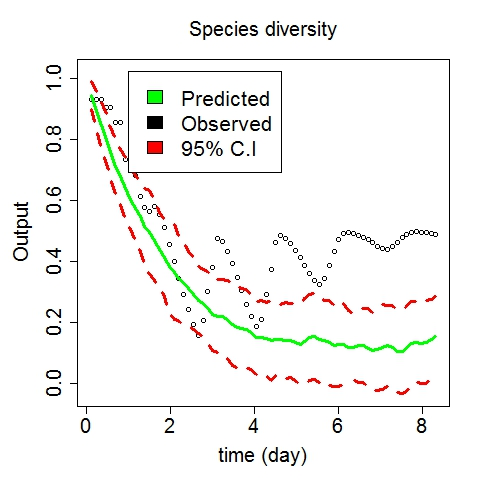
\includegraphics[width=1\textwidth]{p1d/p1d_1}
%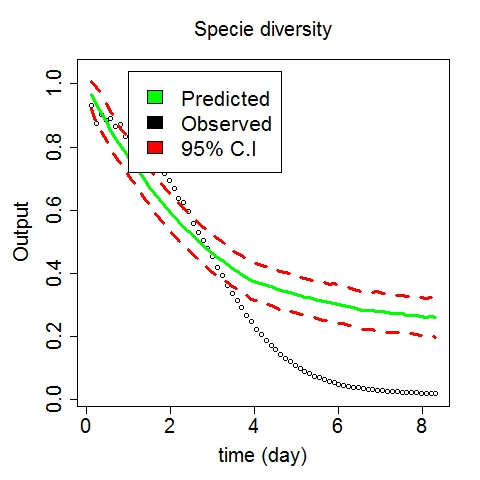
\includegraphics[width=1\textwidth]{p2/p2_1}
%\caption{$\lim_{\delta \to \infty}$}
\end{subfigure}\hspace*{-.5em}
\centering
\begin{subfigure}[b]{.6\textwidth}
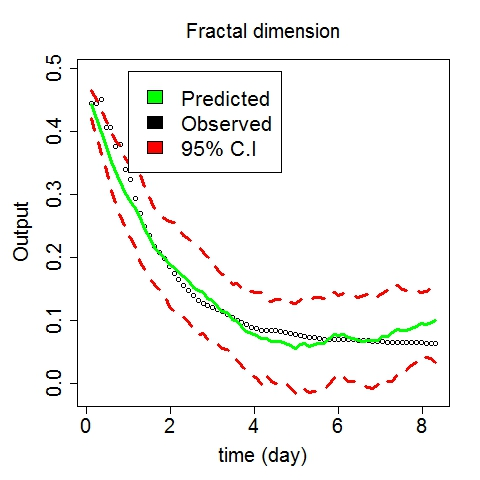
\includegraphics[width=1\textwidth]{p1d/p1d_3}
%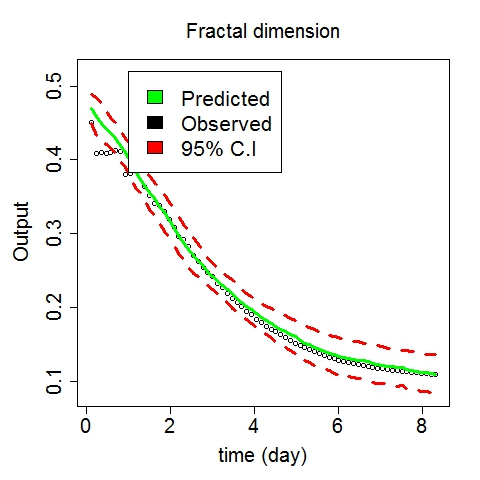
\includegraphics[width=1\textwidth]{p2/p2_3}%{result2/diag1bb}
%\caption{$\lim_{\delta \to 0}$}
\end{subfigure}\vspace*{-0.4em}
\begin{subfigure}[b]{.6\textwidth}
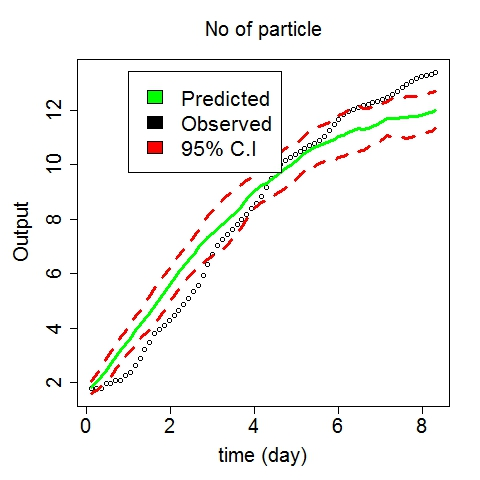
\includegraphics[width=1\textwidth]{p1d/p1d_4}
%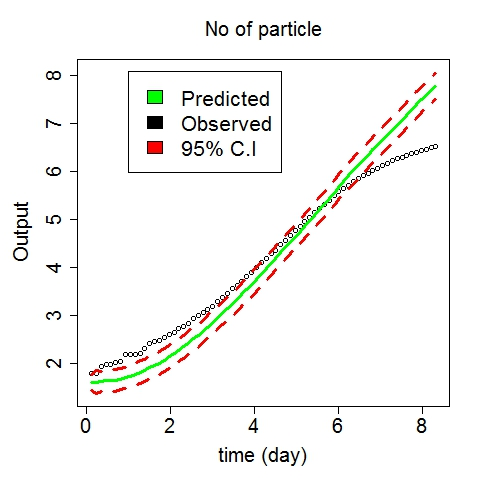
\includegraphics[width=1\textwidth]{p2/p2_4}
%\caption{$\lim_{\delta \to \infty}$}
\end{subfigure}\hspace*{-.5em}
\centering
\begin{subfigure}[b]{.60\textwidth}
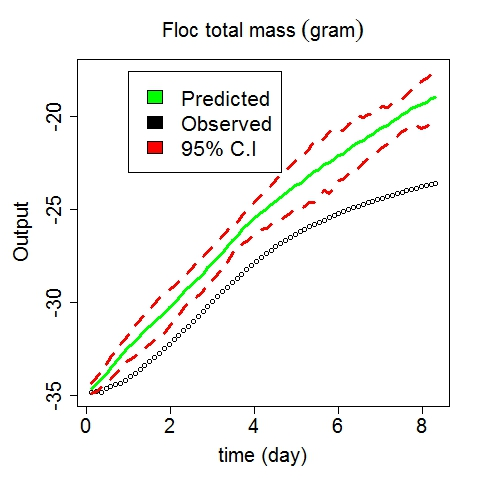
\includegraphics[width=1\textwidth]{p1d/p1d_5}
%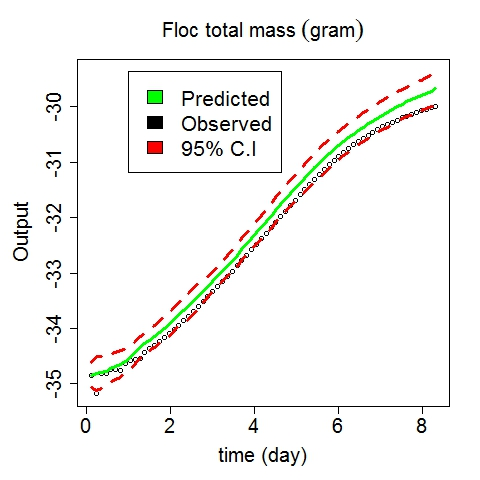
\includegraphics[width=1\textwidth]{p2/p2_5}
%\caption{$\lim_{\delta \to 0}$}
\end{subfigure}\vspace*{-.5em}
\caption[]{Comparison of the emulator performance with simulation data for 4 major outputs from LAMMPS floc simulation (black) and their emulator predictions (green) with 95\% C.I (red). Note: the bottom plots of number of particle and floc total mass are in logarithm scale}\label{ress1}
\end{figure}

Suppose at time step $t$, the LAMMPS output is written in the form 
\begin{equation}
\by_t=f(\bx_t,\by_{t-1}),
\end{equation}
where $\by_{t-1}$ is the state vector at the previous time step, $\bx_t$ are the input at time $t$ which includes the model parameters, forcing and initial conditions as described earlier. We summarise the individual particle at the microscale to a large (mesoscale) as a floc or biofilm. We consider emulation of interested properties of floc and biofilms which are summarised by aggregating the entire individual microbe at each time step. The number of particles $n$ at each time slice varies across the design points as stated earlier. The data is subdivided into two groups. We use 280 data points to build the emulator and use remaining left-out 20 data points to test the performance of the emulator. 
In our training set, we are expected to have about $~20160$ ($280\times 72$) observations for each characterised output. We note that there are some points in our training set where we have incomplete time series of the simulation. The incomplete simulation occurs as a result of the large value of growth rate parameter that is responsible for making the particles grow too rapidly and filled the entire simulation box. This often generates segmentation error and makes the simulation stop earlier. 

A cokriging model could not be applied directly to the entire data because of the computational difficulty of this large sample size coupled with a large number of parameters (33, including initial state variable) to be estimated. We know kriging algorithm scales cubically with the number of observations $O(N^3)$, which is not feasible for our present data. To proceed, we subsample 4500 observations randomly for each output to reduce the computational load. 

Gaussian processes regression (kriging) is prone to numerical problems because of an ill-conditioned covariance matrix. This problem is more pronounced in the cokriging algorithm we used in this study. To reduce the severity of this issue,  we use an exponential covariance function for each output and standardize our input data to range in $[0,1]$.  This transformation will also eliminate the unit of measurement and enable us to get better parameter estimates of covariance functions. 

The histograms of total mass and number of particle in a given floc are displayed in Figure \ref{hist} of the Introductory section. There is a significant degree of skewness and high variance in their patterns, so we log-transformed these two outputs to reduce their skewness and make the data more interpretable to meet our model assumptions. The scatter plots of some of the output data sets (not shown) show a few extreme data points which we exclude from the training data before we fit the model.

We apply the cokriging model to train the resulting data for the characterised outputs (see section \ref{out1}) to produce a single step emulator. We then implement the single-step emulator repeatedly using equations \ref{cokmean} and \ref{cokvar} derived from the normal approximation until time $t=72$ is reached. Because of the stochasticity in the simulation, we fit a heteroscedastic cokriging straightaway by incorporating the empirical variance derived from the replicates as noise in the mean response emulator. This approach will ensure joint predictions of both the mean and variance thus making the data estimation more robust, unlike in \citet{pd26} and \citet{pd22} where an independent GPs is performed on the mean and variance. 

We also fit a separate kriging model for each of the outputs to compare their performance with the cokriging. To test the overall performance of the single-step emulator, we run the emulator for the entire 20 sets and compute the proportion of variance explained by each model outputs. Some results are given below.

Having built the dynamic emulator, we assess the performance of the dynamic emulator by comparing emulator predictions with the simulation data for four different characterised outputs from floc. The cross-validation results are reported in Figures (\ref{ress1},\ref{ress2},\ref{ress3}), they are based on some of the left out 20 design points that were not used to build the emulator. Figure \ref{ress1} gives time series plots showing the pattern of change in the outputs over some days. The plots demonstrate the ability of our dynamic emulator to propagate the chosen outputs forward by applying the emulator iteratively to desired time point. 

Each of the output is plotted against time. The top-left corner is the plot for the species diversity, an index which represents the abundance of different microbial species in a population (floc aggregates). We can see a gradual decreasing in trend over time for simulation data, and this is expected because the species interacts with its environment and other particles within the floc and also compete together for available nutrients. In this study, we know that the HET microbes compete with both AOB and NOB for resources and easily outcompeted and dominate at the end due to higher growth rates and anoxic reactions of HET as compared to AOB and NOB, this often result in loss of some species. 

The species diversity emulator produces similar pattern to the simulation data although after day "3" the emulator deviates from the usual trend but not significantly. This inability of the emulator to capture the entire trend could be further explained by the other plots in Figure \ref{div} in Appendix 4. The plots indicate different temporal behaviours for the species diversity; this could potentially complicate the modelling and ability of the emulator to capture its entire emerging patterns that could degrade the emulator performance over time which suggests that it has not learnt the complete behaviour. 

However, the plots for other outputs are relatively well predicted. The plot of the fractal dimension is shown in the top-right corner shows similar decreasing pattern like species diversity. The values of fractal dimension can be used as a standard for comparing the biological experiments against the theories. The emulator for the fractal dimension predicts the temporal behaviour relatively well, almost all the points lie within the 95\% C.I. The predicted confidence bands remain very small. There is a general increasing trend in the bottom plots for a log-transformed number of particle and the total mass of the floc. 

We note that the shape, size and structure of biofilms and floc are essential operation parameters in the management of wastewater. These characterised physical properties are quite significant in the removal efficiency of solid particles as impurities once they are formed from in wastewater treatment processes.

Figure \ref{ress2} shows a comparison between the probability density function of the simulated and emulated species diversity, fractal dimension, number of particles and the total mass of the floc. The predicted density by the emulator (green) for these outputs are relatively close to the simulation data. The degree of similarity of the distributions reflects the accuracy of the dynamic emulation. The exception is species diversity, which mainly shows over predictions in some area.
The distributions for each output have a single major peak. Moreover, the density of total mass and number of particle have a further minor peak making it bimodal in nature. The skewness of the density function also varies markedly with each output. The density plots for species diversity and fractal dimensions are related. 

\begin{figure}[!ht]
\begin{subfigure}[b]{.6\textwidth}
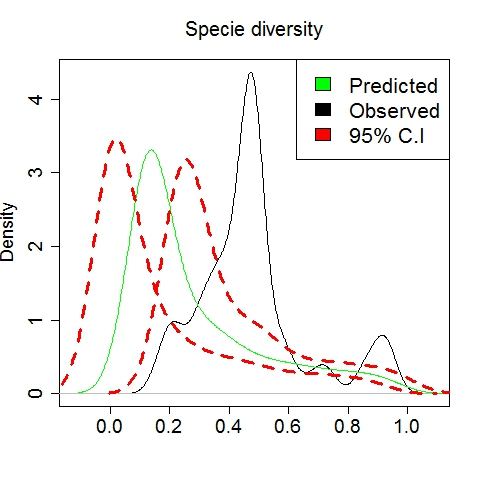
\includegraphics[width=1\textwidth]{p1a1/p1a1_1}
%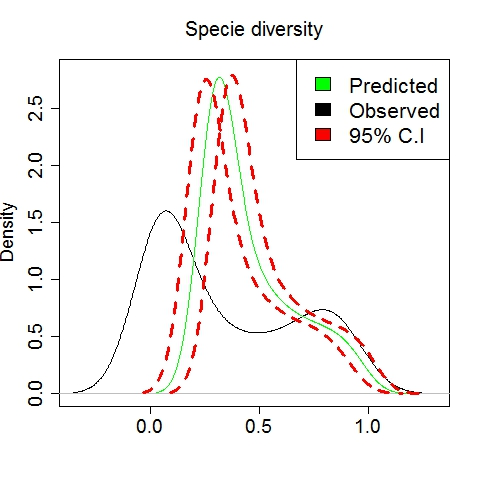
\includegraphics[width=1\textwidth]{p2/p1_1}
%\caption{$\lim_{\delta \to \infty}$}
\end{subfigure}\hspace*{-.5em}
\centering
\begin{subfigure}[b]{.60\textwidth}
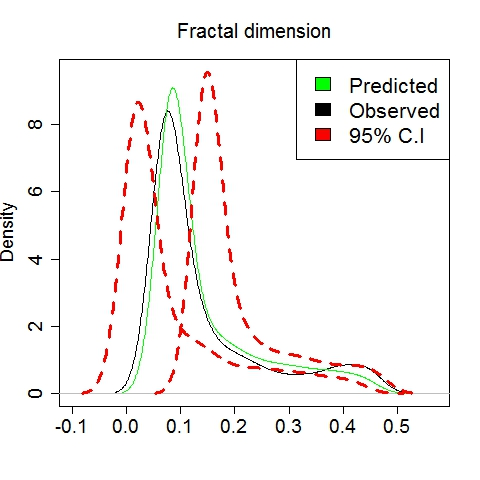
\includegraphics[width=1\textwidth]{p1a1/p1a1_3}
%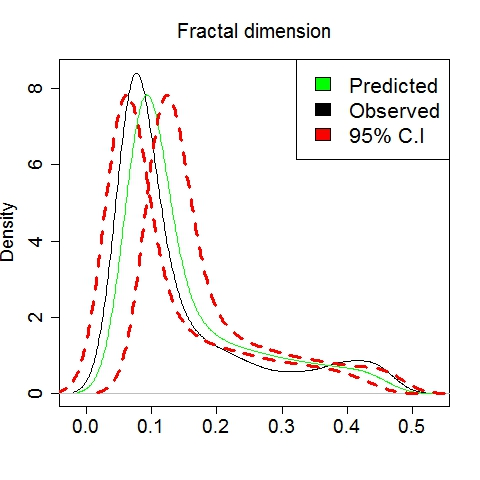
\includegraphics[width=1\textwidth]{result2/tp1_3}
%\caption{$\lim_{\delta \to 0}$}
\end{subfigure}\vspace*{-.5em}
\begin{subfigure}[b]{.6\textwidth}
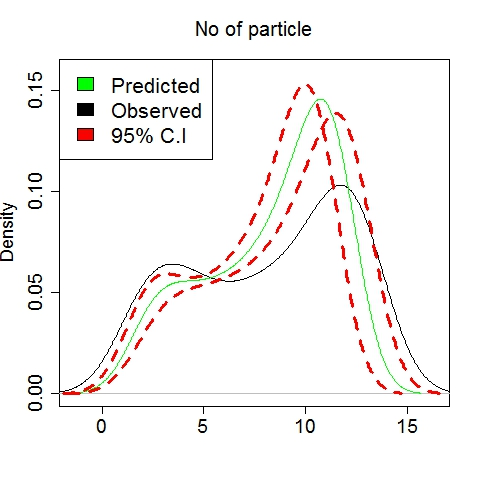
\includegraphics[width=1\textwidth]{p1a1/p1a1_4}
%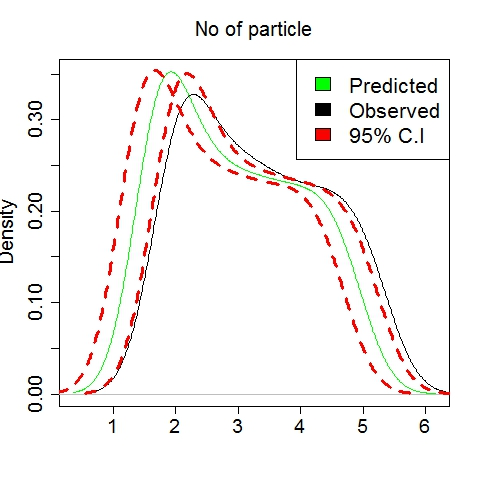
\includegraphics[width=1\textwidth]{result2/tplot1e_4}%{result2/diag1bb}
%\caption{$\lim_{\delta \to \infty}$}
\end{subfigure}\hspace*{-.5em}
\centering
\begin{subfigure}[b]{.60\textwidth}
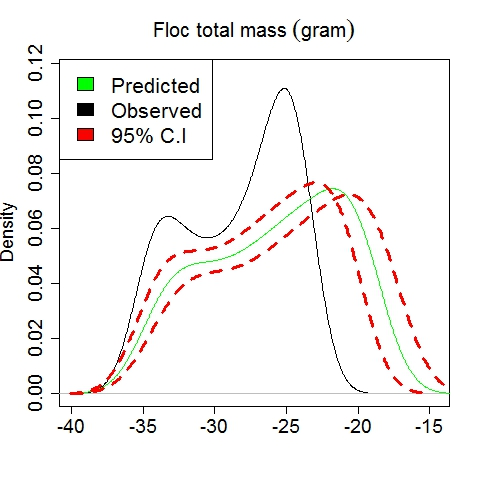
\includegraphics[width=1\textwidth]{p1a1/p1a1_5}
%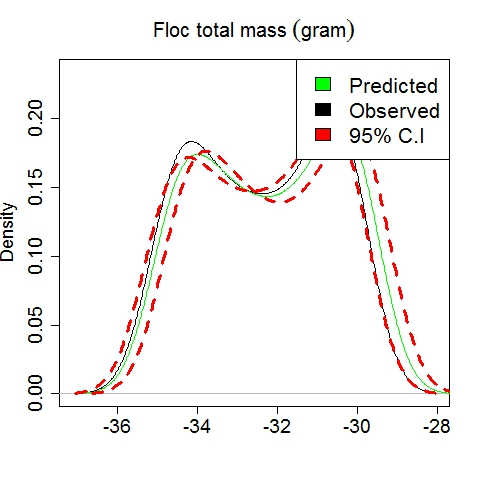
\includegraphics[width=1\textwidth]{p2/p1_5}
%\caption{$\lim_{\delta \to 0}$}
\end{subfigure}\vspace*{-.5em}
\caption[]{Emulator crossvalidation: probability density function for 4 major outputs from LAMMPS floc simulation and their emulator predictions with 95\% C.I. Note: the bottom plots of number of particle and floc total mass are in logarithm scale}\label{ress2}
\end{figure}


\begin{table*}[!Ht]
\caption{Cross-validated proportion of variance $\rho$  and root mean squared error RMSE$_{CV}$ showing the performance of the emulators for randomly chosen design points for flocs and biofilms}
\label{alltab}
\begin{tabular}{lcccc}
\hline
%Crop &\multicolumn{2}{c}{$1^{st}$ stage $\rho$}&&  \multicolumn{2}{c}{$2^{nd}$ stage $\rho$}&&\multicolumn{2}{c}{ RMSE$_{CV}$ ($gC/m^2$)}\\
%\cline{2-3} \cline{5-6} \cline{8-9}
&$\rho$& RMSE$_{CV}$\\
\hline
Floc species diversity&-0.81& \\
Floc eqv. diameter& 0.44 & \\
Floc fractal dimension & 0.98& \\
Floc total number of particle &0.97   &\\
Biofilm mean height &0.95   & &\\
Biofilm surface roughness &0.97   & &\\
Biofilm segregation index & 0.82 &&\\
\hline \vspace{-.2in}
\end{tabular}

%{\footnotesize $^1$ Oil=yield$_{max}$[soyabean, rapeseed, sunflower].\\}
\end{table*}


\subsection{Biofilm emulation}
We describe emulation of bacterial biofilms in this section where we apply the same procedure as in the flocs modelling.
The plots show the assessment of our dynamic emulation approach on the floc outputs where the emulators have been used iteratively to capture the evolution of each of the characterised outputs with time. Figure (\ref{ress1}) in the top-left is the species diversity indices for the particle, and top-right is the plot of fractal dimensions often used to quantify the particle morphology.
We can see that the fractal dimensions produced by the simulator and emulator have similar temporal patterns

Computing the surface roughness, average height and segregation index for biofilms of a set of large particles for a longer period as in this study is a very time-consuming. We, therefore, limit our computation for these two critical biofilm parameters to a few time point (less than two days) as shown in Figure \ref{ress3}.
\begin{figure}[!ht]
\begin{subfigure}[b]{.6\textwidth}
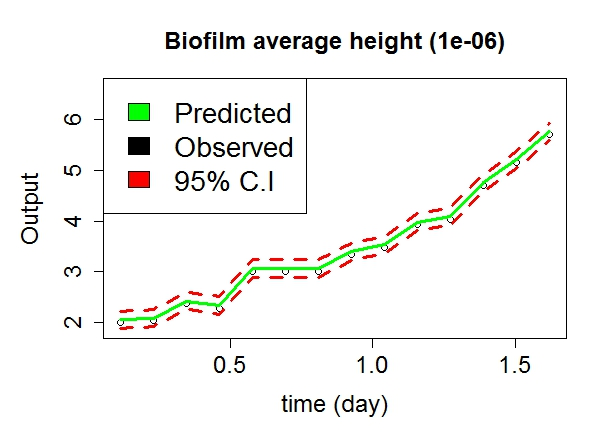
\includegraphics[width=1\textwidth]{result2/height}
%\caption{$\lim_{\delta \to \infty}$}
\end{subfigure}\hspace*{-.5em}
\centering
\begin{subfigure}[b]{.60\textwidth}
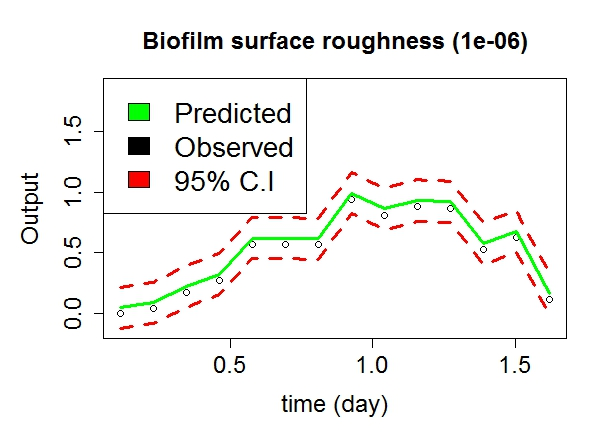
\includegraphics[width=1\textwidth]{result2/roughness}
%\caption{$\lim_{\delta \to 0}$}
\end{subfigure}\vspace*{-.5em}
\caption[]{Comparison of biofilm average height and surface roughness for LAMMPS model and emulator with 95\% C.I}\label{ress3}
\end{figure}

\subsubsection{Sensitivity results}
To have a better understanding of the model parameters, including how their values impact the IB model outputs, a sensitivity analysis of the given parameters to measure their relative importance is performed. The results from this analysis will enhance our understanding of the most contributing input variables to output behaviour. Therefore, we can identify the most influential parameters (out of the 32 parameters we use in this study). Several techniques have been documented in the literature for performing sensitivity analysis \citet{co11}, a popular technique is the Sobol global sensitivity method. This method computes the indices by decomposing the variance up to a specified order \citet{co10}. We use a Bayesian approach for global sensitivity described in \citet{co12} where a Sobol index is estimated based on kriging metamodels. The idea is to incorporate both the uncertainties due to the surrogate modelling and the one due to the numerical evaluations of the variances and covariances involved in the Sobol estimation. 

We sample 1000 observations randomly from a uniform distribution with a range within $[0,1]$, for each of the 32 input variables in Table 1. We computed both the first order sensitivity since we have no quadratic and interaction terms in our model. We then apply a Bootstrapping to compute 95\% confidence intervals on the estimated indices. This procedure was applied to all the eight outputs we consider in this study.


The combined results for both the flocs and biofilms are given below in Figure~ \ref{ress4} for the eight outputs we examine in this paper. The sensitivity analysis clearly indicates that nutrient boundary conditions are the most
critical parameters for predictions of most of the outputs. The outcome result is not surprising because these parameters regulate the distribution and transport of nutrients across the computational domain thus determine the particle growth and division. Also, particle grows when the food is readily available. The substrate boundary concentration "s" with corresponding values 0.26, 0.024, 0.093, 0.043, 0.84, 0.28, 0.88 and  0.40 for the floc total mass, floc equivalent diameter, floc fractal dimension, floc total number of particle, floc species diversity, biofilm average height, biofilm surface roughness and biofilm segregation index respectively, is the dominant variable. The rest are oxygen boundary concentration "o2", nitrate boundary concentration "no3" and ammonia boundary concentration "nh4".The nitrite boundary concentration "no2" is the least sensitive among the nutrient boundary conditions. The next three most sensitive parameters apart from the nutrient concentrations are the HET growth related parameters namely maximum specific growth rate for HET "MumHET", reduction factor in anoxic conditions "etaHET" and  carbon source affinity for HET "KsHET"

\begin{figure}[!ht] 
%\begin{subfigure}[h]{.85\textwidth}
%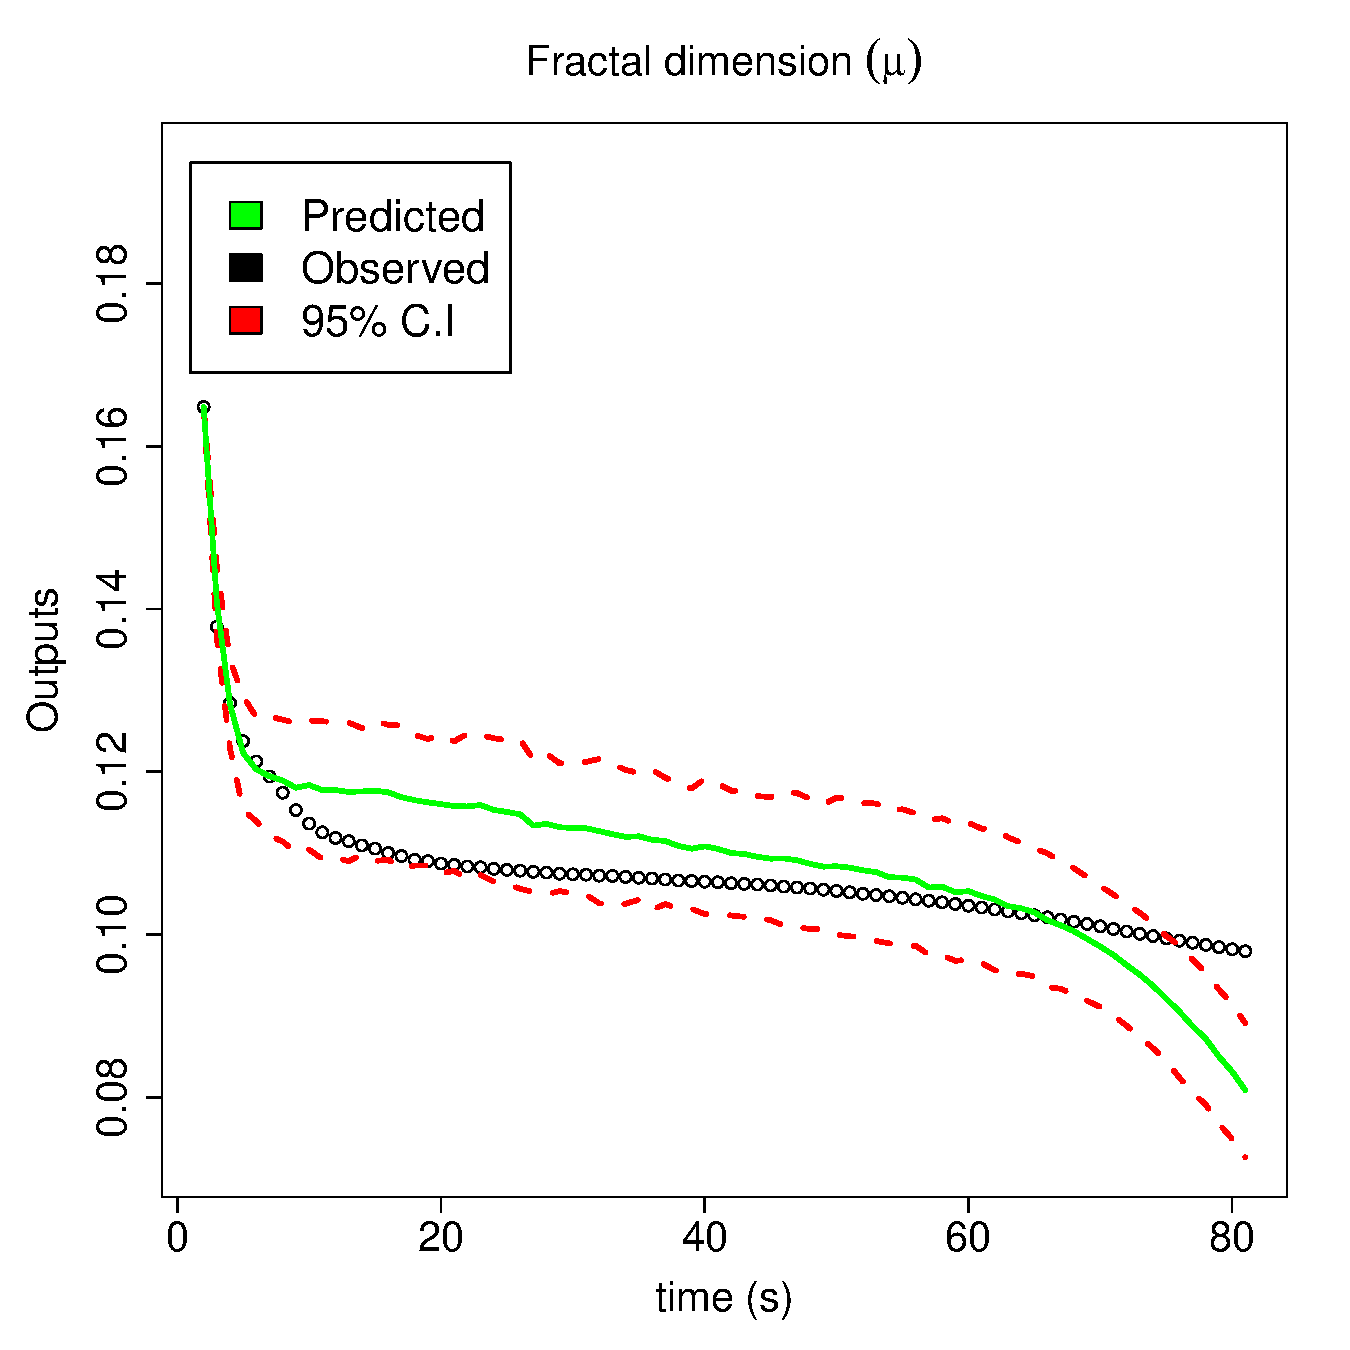
\includegraphics[width=.72\textwidth]{result5/tplot1_1}
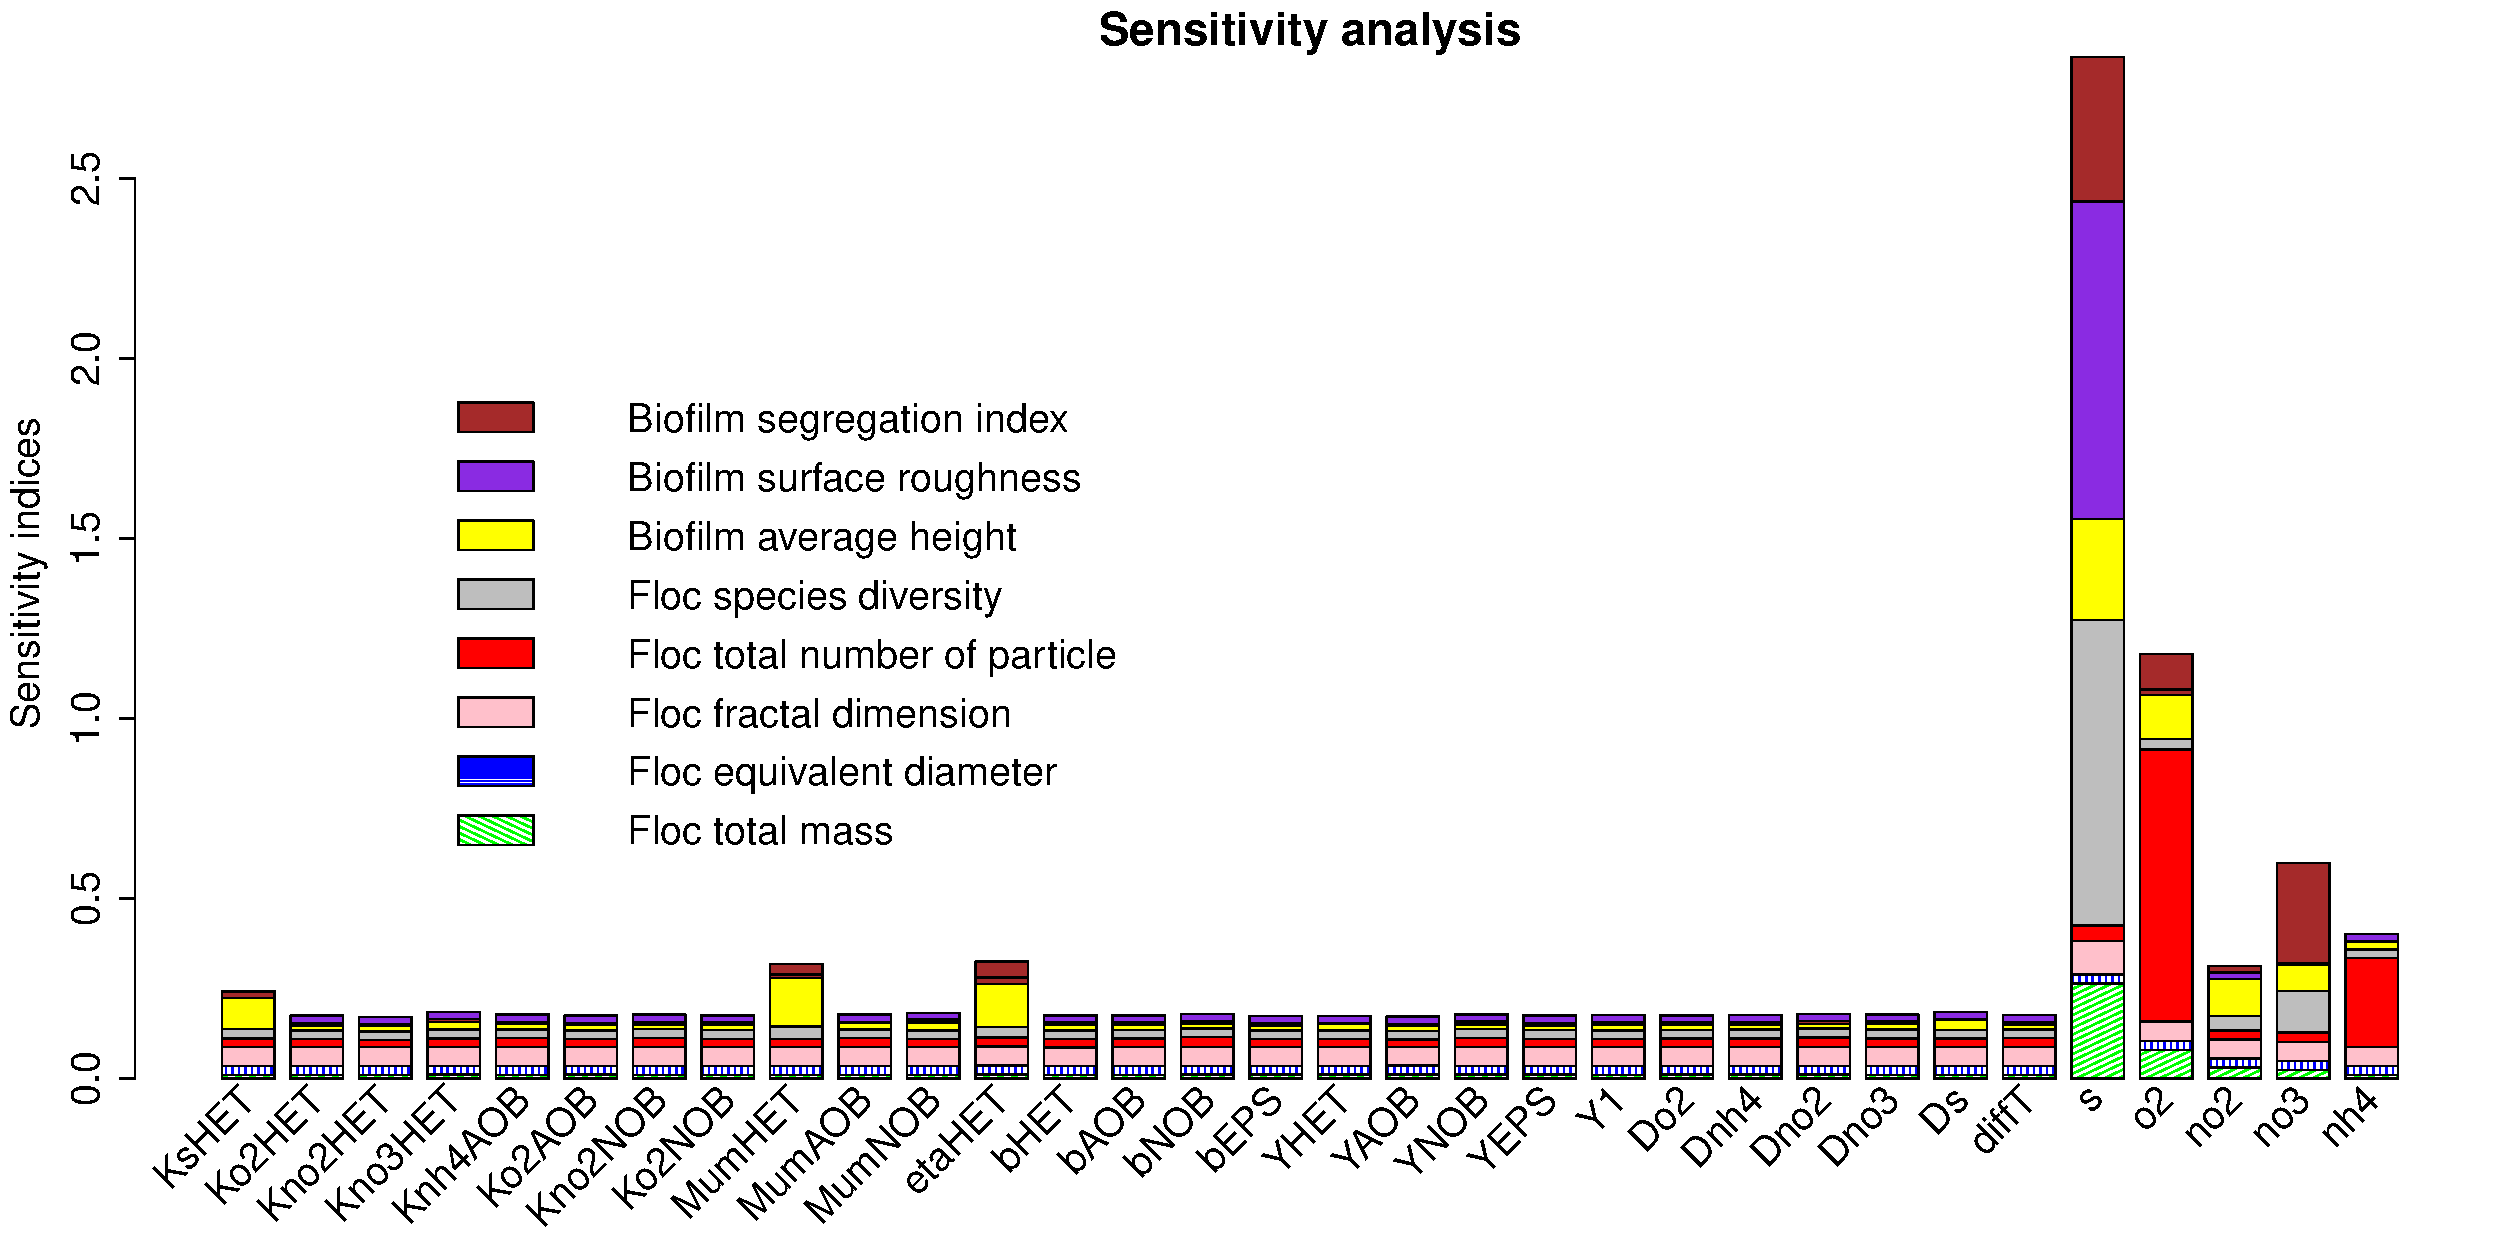
\includegraphics[width=1.1\textwidth]{result2/sens_plot1}
%\end{subfigure}\vspace*{-.99em}
\caption[]{Barplots showing the sensitivity indices for the eight characterized outputs from LAMMPS model.}\label{ress4}
\end{figure}


\section{Discussion}
This paper has shown that cokriging technique can be effectively applied to model a dynamic simulation model while incorporating the noise in the form of empirical variances derived from the replicate observations. We observe that the performance of the single step emulators using it iteratively to capture the underlying dynamics of output behaviours of IB model depend hugely on the initial conditions (initial state variables at time $t_0$) and sample size we take when applying the normal approximation. For the results presented in this paper, we restrict to just 100 samples because of the expense of running the emulator repeatedly. Another critical issue is the evaluation of ill-conditioned covariance parameters which we encounter so often in this analysis because of closely spaced design points. We have reduced the severity of the problem by using an exponential covariance function. We also standardise our input data to range in $[0,1]$.  This transformation also helps to eliminate the effect of measurement units and enable us to get better parameter estimates of covariance functions. Other related challenges we encounter during the emulation are. Overall, the performance of these single-step emulators applying to propagate the state variable forward with time is relatively good.

However, we can also emulate a complete multi-step run of the computer model. One of the ways to proceed with this according to \citet{pd14} is to treat the problem as a multivariate output simulator and develop a multi-output emulator where the dimension of the output space is given as $T$. Closely related to this approach, is to build one single-output emulator that incorporates time as an additional input to the emulator such that $\by_t = f(\bx,t)$, where the training data for building emulator consists $nT$ data points. The limitation of this approach is that it is inefficient in practice because the dimension of the data becomes vast which introduces additional computational difficulty and thus not appropriate for the simulation study in this paper. 
Another alternative is to emulate each time step, which produces an emulator that is peculiar to a particular time step, an approach that assumes independence between the time steps. This method was used in \citet{pd27} but is not suitable for our present data. Here, we are interested in the dynamic behaviours over temporal space, and specifically for using an emulator for making multiple-step ahead predictions. 

%The reason for applying the GP on residual from model results instead of the simulation data. Our simulation data for both crops and climate are high-dimensional gridded global data that cannot be modelled directly by GP. Several approximation techniques have been developed to handle multi-dimensional data. For instance, a low-rank approximation of the Gram matrix was described in \cite{q10,q11}. The use of subsets of regressors and subsets of data to reduce the computational burden of the GP inversion for a large data matrix was investigated by \cite{q12,q13,q14}. The following studies used Bayesian techniques for emulating high-dimensional data \cite{q28,q29,q22,q23,qq}. A good emulator must be as fast as possible to allow for relatively quick evaluation of many scenarios which are not feasible with these techniques. Therefore, the Bayesian procedures used in the studies mentioned above cannot be directly applied to handle large dimensional and high-resolution crop data in this study. 

%Another way to resolve our problem is to treat each spatial point as a GP and then emulate each grid cell individually a technique implemented in \cite{q62} and \cite{q64}. However, this option is intractable since we have 59199 grid points meaning that about 236,796 emulators have to be constructed and validated for the four crops we are emulating.

%\newpage
\section{Conclusion}
In this paper, we demonstrate a new concept of making inference about the parameters of the emulator using a GP regression that is based upon multifidelity cokriging technique. This concept relies on the assumption that characterised outputs from the IB model can form a different level of codes. Stochasticity in the simulation is treated by incorporating noise in the form of empirical variances derived from the replicates. Our approach combines the two-stage technique proposed in \citet{pd11} and \citet{qwole} as a single step. We have presented a simple statistical method for emulating the underlying physical dynamics of the major characterised outputs of the IB model simulations of microbial growth. In modelling our microscale simulation data as flocs and bacteria biofilms, we reduced the complexity of the computation by aggregating spatially from a fine (individual microbes) to a more coarse resolution as flocs and biofilms. We assume that the aggregation will reduce the complexity and structure of the global trend component of the emulator. 

These emulators are much faster to run compared to the simulation model. The IB model simulation implemented within LAMMPS is computationally expensive to run, while these emulators give results almost instantaneously.
Under different parameter combinations, it takes an average of between $8-10$ hours to simulate the growth of the particles for about eight days at 20s timestep on Linux cluster machine. Apart from the computation time requires for fitting the single-step emulator, it takes $<2$ min to apply the emulator iteratively to generate the corresponding trajectories of the characterised outputs. This shows approximately 240-fold increase in computational efficient.

\begin{acknowledgements}
The work has been supported by Newcastle University under the Frontiers in Engineering Biology (NUFEB) project.
%If you'd like to thank anyone, place your comments here
%and remove the percent signs.
%\end{acknowledgements}

% BibTeX users please use one of
%\bibliographystyle{spbasic}      % basic style, author-year citations
%\bibliographystyle{spmpsci}      % mathematics and physical sciences
%\bibliographystyle{spphys}       % APS-like style for physics
%\bibliography{}   % name your BibTeX data base

% Non-BibTeX users please use
%\begin{thebibliography}{}
%\end{thebibliography}


%\begin{thebibliography}{94}
%\cleardoublepage
%\phantomsection
%\bibliographystyle{plain}


\begin{thebibliography}{94}
%\cleardoublepage
%\phantomsection
\bibliographystyle{plain}
\bibitem[Currin et al.(1991)]{pd1} Currin, C., Mitchell, T.J., Morris, M.D., and Ylvisaker, D. (1991). Bayesian Prediction of Deterministic Functions, With Applications to the Design and Analysis of Computer Experiments. {\it Journal of the American Statistical Association}, $86(416), 953-963$. 

\bibitem[Martin \& Simpson(2004)]{pd2} Martin, J. D., \& Simpson, T. W. (2004). On the use of kriging models to approximate deterministic computer models. {\it In ASME 2004 International Design Engineering Technical Conferences and Computers and Information in Engineering Conference}, $481-492$.

\bibitem[Osio et al.(1996)]{pd3} Osio, I.G. and Amon, C.H. (1996). An Engineering Design Methodology with Multistage Bayesian Surrogate and Optimal Sampling. {\it Research in Engineering Design}, $8(4), 189-206$.

\bibitem[Sacks et al.(1989)]{pd4} Sacks, J., Welch, W., Mitchell, T., Wynn, H. (1998). Design and analysis of computer experiments. {\it Statistical Science}, $4(4), 409-435$.

\bibitem[Santner et al.(2003)]{pd5} Santner, T., Williams, B., Notz, W. (2003). The Design and Analysis of Computer Experiments. Springer.

\bibitem[Li \& Sudjianto(2005)]{pd6} Li, R., \& Sudjianto, A. (2005). Analysis of computer experiments using penalized likelihood in gaussian kriging models. {\it Technometrics}, $47(2), 111-120$.

\bibitem[Andrianakis \& Challenor(2009)]{pd7} Andrianakis, Y., \& Challenor, P. G. (2009). Parameter estimation and prediction using gaussian processes. {\it Technical report}, MUCM Technical report 09/05, University of Southampton.

\bibitem[Roustant et al.(2012)]{pd8} Roustant, O., Ginsbourger, D., \& Deville, Y. (2012). DiceKriging, DiceOptim: Two R packages for the analysis of computer experiments by kriging-based metamodeling and optimization.

\bibitem[Park \& Baek(2001)]{pd9} Park J.S., \& Baek, J. (2001). Efficient Computation of Maximum Likelihood Estimators in a
Spatial Linear Model with Power Exponential Covariogram. {\it Computer Geosciences}, $27, 1-7$.

\bibitem[Hankin(2005)]{pd10} Hankin, R. K. (2005). Introducing BACCO, an R package for Bayesian analysis of computer code output. {\it Journal of Statistical Software}, $14(16), 1-21$.

\bibitem[O'Hagan(2006)]{pd11} O'Hagan, A. (2006). Bayesian Analysis of Computer Code Outputs: A Tutorial. {\it Reliability Engineering and System Safety}, $91, 1290-1300$.

\bibitem[Conti et al.(2009)]{pd12} Conti, S., Gosling, J. P., Oakley, J. E., \& O'hagan, A. (2009). Gaussian process emulation of dynamic computer codes. {\it Biometrika}, asp028.

%\bibitem[Conti {\em et al}.(2004)]{pd13} Conti, S., Anderson, C. W., Kennedy, M. C., \& O’Hagan, A. (2004). A Bayesian analysis of complex dynamic computer models. {\it In Proc. of the 4th International Conference on Sensitivity Analysis of Model Output}.

\bibitem[Conti {\em et al}.(2010)]{pd14} Conti, S., \& O’Hagan, A. (2010). Bayesian emulation of complex multi-output and dynamic computer models. {\it Journal of statistical planning and inference}, $140(3), 640-651$.

\bibitem[Bhattacharya(2007)]{pd15} Bhattacharya, S. (2007). A simulation approach to Bayesian emulation of complex dynamic computer models. {i\t Bayesian Analysis}, $2(4), 783-815$.

%\bibitem[Kennedy {\em et al}.(2001)]{pd16} Kennedy, M.C., \& O'Hagan, A. (2001). Bayesian calibration of computer models. {\it Journal of the Royal Statistical Society}. Series B, Statistical Methodology, $425-464$.

\bibitem[Azman \& Kocijan (2005)]{pd17} Azman, K., \& Kocijan, J. (2005). Comprising prior knowledge in dynamic gaussian process models. {\it In Proceedings of the International Conference on Computer Systems and Technologies-CompSysTech}, Vol. 16(17.6).

\bibitem[Kleijnen(2009)]{pd18} Kleijnen, J. P. (2009). Kriging metamodeling in simulation: A review. {\it European Journal of Operational Research}, $192(3), 707-716$.

\bibitem[Kleijnen \& Simpson(2005)]{pd19} Martin, J. D., \& Simpson, T. W. (2005). Use of kriging models to approximate deterministic computer models. {\it AIAA journal}, $43(4), 853-863$.

\bibitem[Kleijnen \& Mehdad(2014)]{pd20} Kleijnen, J. P., \& Mehdad, E. (2014). Multivariate versus univariate kriging metamodels for multi-response simulation models. {\it European Journal of Operational Research}, $236(2), 573-582$.

\bibitem[Boukouvalas {\em et al}.(2009)]{pd21} Kleijnen, J. P. (2009) Boukouvalas, A., Cornford, D., \& Singer, A. (2009). Managing uncertainty in complex stochastic models: {\it Design and emulation of a rabies model. In 6th St. Petersburg Workshop on Simulation}, (pp. 839-841).

\bibitem[Kersting {\em et al}.(2007)]{pd22} Kersting, K., Plagemann, C., Pfaff, P., \& Burgard, W. (2007). Most likely heteroscedastic Gaussian process regression. {\it In Proceedings of the 24th international conference on Machine learning}, (pp. 393-400). ACM.

\bibitem[Kleijnen \& Beers(2005)]{pd23} Kleijnen, J.P., \& Van Beers, W.C. (2005). Robustness of kriging when interpolating in random simulation with heterogeneous variances: Some experiments. {\it European Journal of Operational Research}, $165(3), 826-834$.

\bibitem[Bates {\em et al}.(2006)]{pd24} Bates, R. A., Kenett, R. S., Steinberg, D. M., \& Wynn, H. P. (2006). Achieving robust design from computer simulations. {\it Quality Technology and Quantitative Management}, $3(2), 161-177$.

\bibitem[Bates {\em et al}.(1997)]{pd25} Goldberg, P. W., Williams, C. K., \& Bishop, C. M. (1997). Regression with input-dependent noise: A Gaussian process treatment. {\it Advances in neural information processing systems}, $10, 493-499$.

\bibitem[Henderson {\em et al}.(2012)]{pd26} Henderson, D. A., Boys, R. J., Krishnan, K. J., Lawless, C., \& Wilkinson, D. J. (2012). Bayesian emulation and calibration of a stochastic computer model of mitochondrial DNA deletions in substantia nigra neurons. {\it Journal of the American Statistical Association}.

\bibitem[Boukouvalas {\em et al}.(2014)]{pd27} Boukouvalas, A., Sykes, P., Cornford, D., \& Maruri-Aguilar, H. (2014). Bayesian precalibration of a large stochastic microsimulation model. {\it Intelligent Transportation Systems, IEEE Transactions on}, $15(3), 1337-1347$.

\bibitem[Kleijnen \& Mehdad(2012)]{pd28} Kleijnen, J., \& Mehdad, E. (2012). Kriging in multi-response simulation, including a Monte Carlo laboratory. {CentER Discussion Papers Series}, (2012-039).

\bibitem[Jarvis {\em et al}.(2005)]{l3} Jarvis, P., Jefferson, B., \& Parsons, S. A. (2005). Measuring floc structural characteristics. {\it Reviews in Environmental Science and Bio/Technology}, $4(1-2), 1-18$.

\bibitem[Frazer {\em et al}.(2013)]{l4}  Fraser, C. E., McIntyre, N., Jackson, B. M., \& Wheater, H. S. (2013). Upscaling hydrological processes and land management change impacts using a metamodeling procedure. {\it Water Resources Research}, $49(9), 5817-5833$.

 \bibitem[Wheater {\em et al}.(2008)]{l8} Wheater, H.S., B. Reynolds, N. McIntyre, M. Marshall, B. Jackson, Z. Frogbrook, I. Solloway, O. J. Francis, and J. Chell (2008). Impacts of upland land management on flood risk: Multi-scale modelling methodology and results from the Pontbren experiment, {\it FRMRC Res. Rep. UR}, 16, 163 pp., Imp. Coll. \& CEH Bangor, London, U.K.

 \bibitem[Van {\em et al}.(2009)]{l9} Van Oijen, M., Thomson, A., \& Ewert, F. (2009). Spatial upscaling of process-based vegetation models: An overview of common methods and a case-study for the UK. Methods, 1(3).
 
\bibitem[Ofiteru {\em et al}.(2014)]{l11} Ofiteru, I. D., Bellucci, M., Picioreanu, C., Lavric, V., \& Curtis, T. P. (2014). Multi-scale modelling of bioreactor–separator system for wastewater treatment with two-dimensional activated sludge floc dynamics. {\it Water research}, $50, 382-395$.

%\bibitem[Hankin(2005)]{pd32} Hankin, R. K. (2005). Introducing BACCO, an R package for Bayesian analysis of computer code output. {\it Journal of Statistical Software}, $14(16), 1-21$.

%%%%%%%%%%%%%%%%%




\bibitem[Higdon {\em et al}.(2008)]{q23} Higdon, D., Gattiker, J., Williams, B. \& Rightley, M. (2008). Computer model calibration using high-dimensional output. {\it Journal of the American Statistical Association}, $103, 570-583$.


\bibitem[Kennedy {\em et al}.(2001)]{45} Kennedy, M.C. \& O'Hagan, A. (2001). Bayesian calibration of computer models. {\it Journal of Royal Statistical Society}, series B, $63(3), 425-464$.

\bibitem[Kennedy {\em et al}.(2006)]{q17} Kennedy, M. C., Anderson, C. W., Conti, S., and O'Hagan, A. (2006). Case studies in Gaussian process modelling of computer codes. {\it Reliability Engineering \& System Safety}, $91, 1301-1309$.

%\bibitem[Kennedy {\em et al}.(2008)]{46} Kennedy, M.C. {\em et al}. (2008). Quantifying uncertainty in the biospheric carbon flux for England and Wales. {\it Journal of the Royal Statistical Society}, Series B, $171, 109-135$.




\bibitem[Oakley(1999)]{q35} Oakley, J. (1999). Bayesian Uncertainty Analysis For Complex Computer Codes. Ph.D. thesis, University of Sheffield.

\bibitem[Oakley \& O'Hagan(2002)]{60} Oakley, J. and O'Hagan, A. (2002). Bayesian inference for the uncertainty distribution of computer model outputs. {\it Biometrika}, $89, 769-784$.

\bibitem[Oakley \& O'Hagan(2004)]{q5} Oakley, J. E. and O'Hagan, A. (2004). Probabilistic sensitivity analysis of complex models: a Bayesian approach.{\it Journal of Royal Statistical Society}, $66B, 751-769$.


\bibitem[Oyebamiji {\em et al}.(2015)]{qwole} Oyebamiji, O.K., Edwards, N.R., Holden, P.B., Garthwaite, P.B., Schaphoff, S., and Gerten, D. (2015). Emulating global climate change impacts on crop yields. {\it Statistical Modelling}, 1471082X14568248.

%\bibitem[O'Hagan(2006)]{l5} O'Hagan, A. (2006). Bayesian Analysis of Computer Code Outputs: A Tutorial. {\it Reliability Engineering and System Safety}, $91, 1290-1300$.

\bibitem[Higdon {\em et al}.(2008)]{l6} Higdon, D., Gattiker, J., Williams, B. \& Rightley, M. (2008). Computer model calibration using high-dimensional output. {\it Journal of the American Statistical Association}, $103, 570-583$.

\bibitem[Quinonero-Candela \& Rasmussen(2005)]{q47} Quinonero-Candela, J., \& Rasmussen, C. E. (2005). A unifying view of sparse approximate Gaussian process regression. {\it The Journal of Machine Learning Research}, $6, 1939-1959$.


\bibitem[Rasmussen \& Williams(2006)]{q10} Rasmussen, C.E. and Williams, C.K.I. (2006). Gaussian Processes for Machine Learning, the MIT Press.


%\bibitem[Rougier(2007)]{68} Rougier, J.C. (2007). Probabilistic inference for future climate using an ensemble of climate model evaluations. {\it Climate Change}, $81, 247-264$.

%\bibitem[Rougier(2008)]{q28} Rougier, J. (2008). Efficient emulators for multivariate deterministic functions. {\it Journal of Computational and Graphical Statistics}, $17(4), 827-843$.

%\bibitem[Rougier {\em et al}.(2009)]{q29} Rougier, J., Guillas, S., Maute, A., \& Richmond, A. D. (2009). Expert knowledge and multivariate emulation: The thermosphere–ionosphere electrodynamics general circulation model (TIE-GCM). {\it Technometrics}, $51(4), 414-424$.

\bibitem[Sacks {\em et al}.(1989)]{q7} Sacks, J., Welch, W., Mitchell, T., Wynn, H. (1998). Design and analysis of computer experiments. {\it Statistical Science}, $4(4), 409-435$.

%\bibitem[Sacks {\em et al}.(2010)]{r8} Sacks,W.J., Deryng, D., Foley, J.A., Ramankutty, N. (2010). Crop planting dates: an analysis of global patterns. {\it Global Ecology and Biogeography}, $19, 607–620$.

\bibitem[Santner {\em et al}.(2003)]{70} Santner, T., Williams, B., Notz, W. (2003). The Design and Analysis of Computer Experiments. Springer.

%\bibitem[Shi {\em et al}.(2005)]{q18} Shi, J.Q., Murray-Smith, R. and Titterington, D.M. (2005). Hierarchical Gaussian Process mixtures for regression. {\it Statistics and Computing}, $15, 31-41$.

\bibitem[Wilkinson(2010)]{80} Wilkinson, R.D., in: Biegler {\em et al}. (Eds.) (2010). Large-Scale Inverse Problems and Quantification of Uncertainty. {\it John Wiley \& Sons}, New York.

\bibitem[Young {\em et al}.(2011)]{83} Young, P.C. and Ratto, M. (2011). Statistical emulation of large linear dynamic models. {\it Technometrics}, $53(1), 29-43$.
%%%%%%19-05-2016
\bibitem[Le Gratiet (2013)]{co1} Le Gratiet, L. (2013). Bayesian analysis of hierarchical multifidelity codes. SIAM/ASA {\it Journal on Uncertainty Quantification}, $1(1), 244-269$.

\bibitem[Le Gratiet \& Garnier(2014)]{co2} Le Gratiet, L., \& Garnier, J. (2014). Recursive co-kriging model for design of computer experiments with multiple levels of fidelity. {\it International Journal for Uncertainty Quantification}, $4(5).$

\bibitem[Forrester et al.(2007)]{co3} Forrester, A. I., Sobester, A., \& Keane, A. J. (2007). Multi-fidelity optimization via surrogate modelling. {\it In Proceedings of the royal society of london a: mathematical, physical and engineering sciences}, $463(2088), 3251-3269$. The Royal Society.

\bibitem[Kennedy \& O'Hagan(2000)]{co4} Kennedy, M. C., \& O'Hagan, A. (2000). Predicting the output from a complex computer code when fast approximations are available. {\it Biometrika}, $87(1), 1-13$.

\bibitem[Kuya et al.(2011)]{co5} Kuya, Y., Takeda, K., Zhang, X., \& J. Forrester, A. I. (2011). Multifidelity surrogate modeling of experimental and computational aerodynamic data sets. {\it AIAA journal}, $49(2), 289-298$.


\bibitem[Amaral et al.(1997)]{co6} Amaral, A. L., Alves, M. M., Mota, M., \& Ferreira, E. C. (1997). Morphological characterisation of microbial aggregates by image analysis. {\it Proceedings of the $9^th$ Pattern Recorgnition Conference}, $95-100$, Coimbra, 1997.

\bibitem[de Boer et al.(2000)]{co7} de Boer, D. H., Stone, M., \& Levesque, L. M. (2000). Fractal dimensions of individual flocs and floc populations in streams. {\it Hydrological Processes}, $14(4), 653-667$.

\bibitem[Zmeskal et al.(2001)]{co8} Zmeskal, O., Vesely, M., Nezadal, M., \& Buchnicek, M. (2001). Fractal analysis of image structures. {\it Harmonic and Fractal Image Analysis}, $3-5$.

\end{thebibliography}{}





\section*{Appendix 1: Model parameters}
\begin{table}[!ht] 
\caption{List of IB model parameters}\label{mytab1}
\centering
\fbox{
\begin{tabular}{*{2}{c|c|c}}
Index&Parameters& Values\\ 
\hline 
&Affinity variables\\
\hline
1&KsHET &0.01\\
2&Ko2HET & 0.81\\
3&Kno2HET & 0.0003\\
4&Kno3HET & 0.0003\\

5&Knh4AOB & 0.001\\
6& Ko2AOB & 0.0005\\

7&Kno2NOB & 0.0013\\
8&Ko2NOB & 0.00068\\
\hline
&Maximum growth variables\\
\hline
9&MumHET & 0.00006944444\\
10&MumAOB & 0.0000088\\
11&MumNOB & 0.000009375\\
12&etaHET & 0.6\\
\hline
&Decay rates variables\\
\hline 
13& bHET & 0.00000462962\\
14&bAOB & 0.00000127314\\
15&bNOB & 0.00000127314\\
16&bEPS & 0.00000196759\\
\hline
&Yield coefficient variables\\
\hline 
17&YHET & 0.61\\
18&YAOB & 0.33\\
19&YNOB & 0.083\\
20&YEPS & 0.18\\
\hline
&Diffusion coefficient variables\\
\hline 
21&Do2 & 0.000000002\\
22&Dnh4 & 0.0000000014\\
23&Dno2 & 0.0000000012\\
24&Dno3 & 0.0000000012\\
25&Ds & 0.0000000005\\
\hline
&Critical diameter of death\\
\hline 
26&deadDia & 0.0000008\\
27&factor &1.5\\
\hline
&Inlet concentrations (nutrients)\\
\hline \hline
1&sub &0.008 \\
2&no2 & 0.0001\\
3&no3 & 0.0008\\
4&o2 & 0.0008\\
5&nh4 &0.0009\\

\end{tabular}}
\end{table}

%\newpage
%\section*{Appendix 1: GP derivation}

\section*{Appendix 2: Model performance}
We compute the squared differences between the actual floc and biofilms characterized outputs. For instance, for equivalent diameter $d_{eqv}$, as $\by$ and $\bar \by$ and also compute the squared differences between the LAMMPS values and the emulator predictions. The proportion of the variance in the LAMMPS model that is explained by the emulator is given as
%\begin{equation}
\begin{align}\tag{A.1}\label{gaga4}
\rho=1-\left[\frac{\sum\limits_{t=1}^T\sum\limits_{n=1}^N
(\by_{tn}-\bar \by_{tn})^2}
{\sum\limits_{t=1}^T\sum\limits_{n=1}^N
(y_{tn}-\bar y)^2}\right]
\end{align}
and the overall cross-validation root mean squared error (RMSE$_{CV}$) is
\begin{equation}\tag{A.2}\label{gaga4b}
\mbox{RMSE}_{CV}= \left(\sum\limits_{t=1}^8\sum\limits_{n=1}^N
\frac{(\by_{tn}-\bar \by_{tn}^{\star})^2}{(T\times N)} \right)^{1/2}.
\end{equation}

\section*{Appendix 3: MLE of cokriging parameters}
We use a maximum likelihood approach of \citet{co3} and \citet{co4} because of its computational efficiency. The MLE procedure is divided into two categories. Firstly, we consider estimating the parameters $\theta_1=(\bbeta_1,\sigma_1^2,\balpha_1)$ and  $\theta_2=(\bbeta_r,\rho,\sigma_r^2,\balpha_r)$ differently because of the conditional independence that exists between the data $Y_1(x)$ and $Y_2(x)$. Therefore, we can maximize the log-likelihood given below to estimate $\theta_1$
\begin{equation}\tag{A.3}\label{cok3}
-\frac{n_1 log(\sigma_1^2)}{2} -  \frac{1}{2}log(|\Psi_1(\bX_1,\bX_1)|) - \frac{ \Big \{(\by_1-F_1 \bbeta_1)^T \Psi_1(\bX_1,\bX_1)^{-1}(\by_1-F_1 \bbeta_1)\Big\}}{2\sigma_1^2}
\end{equation}
where $|\Psi_1(\bX_1,\bX_1)|$ is the determinant of correlation matrix $\Psi_1(\bX_1,\bX_1)$, by taking the derivative of the equation (\ref{cok3}) with
respect to $\bbeta_1$ and $\sigma_1^2$ and solving for zero, the estimates $\hbbeta_1$ and $\hat\sigma_1^2$ are given respectively as
$$\hbbeta_1=(F_1^T \Psi_1(\bX_1,\bX_1) F_1)^{-1}F_1^T\Psi_1(\bX_1,\bX_1)^{-1}\by_1$$

and $\hat{\sigma_1^2}=\frac{1}{n_1} \Big[(\by_1-F_1\hbbeta_1)^T  \Psi_1(\bX_1,\bX_1)(\by_1-F_1\hbbeta_1)\Big]$.
The alternative way of performing this computation under fully-Bayesian technique of \citet{co1} and \citet{co2} is to marginalise the conditional $\Big(f(.) | \by_1, \bbeta_1, \sigma_1^2, \boldsymbol{\alpha_1}\Big)$ with respect to $\bbeta_1$ and $\sigma_1^2$. 
To estimate $\balpha_1$, we maximize over $\balpha_1$ the concentrated likelihood given below after plugging the values of $\hbbeta$ and $\hat{\sigma_1^2}$ in equation (\ref{cok3}) to give
\begin{equation}\tag{A.4}
-\frac{n_1 log( \hat \sigma_1^2)}{2} -  \frac{1}{2}log(|\Psi_1(\bX_1,\bX_1)|) 
\end{equation}

Secondly, we describe estimation of $\theta_2=(\bbeta_r,\rho,\sigma_r^2,\balpha_r)$. Let $\br=\by_2-\rho \by_1(\bX_2)$ and  $F=[F_2~~~~\rho \by_1(\bX_2)]$,
where $\by_1(\bX_2)$ are the collocated points of $\by_1$ and $\by_2$.
 Therefore, the log-likelihood of $\br|\by_2$ is given as
\begin{equation}\tag{A.5}\label{cok4}
-\frac{n_2}{2} log(\sigma_r^2) -  \frac{1}{2}log(|\Psi_r(\bX_2,\bX_2)|) - \frac{ \Big \{(\br-F \bbeta_r)^T \Psi_r(\bX_2,\bX_2)^{-1}(\br-F\bbeta_r)\Big\}}{2\sigma_r^2}
\end{equation}
$\hbbeta_r=(F^T \Psi_r(\bX_2,\bX_2) F)^{-1}F^T\Psi_r(\bX_2,\bX_2)^{-1}\br$, ~~~~~ $\hat{\sigma_r^2}=\frac{1}{n_2} \Big[(\br-F\hbbeta_r)^T  \Psi_r(\bX_2,\bX_2)(\br-F\hbbeta_r)\Big]$. Again, $\balpha_r$ and $\rho$ are estimated by maximized the restricted log-likelihood derived by substituting values $\hbbeta_r$ and $\hat{\sigma_r^2}$ in equation (\ref{cok4}). The trend and covariance parameters $\balpha_r$ and $\rho$ is computed by using a global optimiser which is based on the extension of the efficient algorithm proposed in \citet{pd9} for likelihood maximization. Further details are provided in \citep{pd8}. The derivation above can be extended to a case where $k>2$ and for $k=1$, our results is equivalent to universal kriging estimate.  %The mean and variance can be estimated by using equation (\ref{cok1}). See futher detail in \citep{co4}.

Due to the stochastic nature of the data we analyse in this paper, we briefly describe the extension of above derivation for the noisy observations, covariance $K=\sigma^2\bC$ is replaced by $ \sigma^2\bC+diag(\btau^2_1,\ldots,\btau^2_n)$ in equations (\ref{man}, \ref{olu2b}) respectively for the kriging predictor, where $\btau^2=\tau^2_1,\ldots,\tau^2_n$ are the noise variances. And for the cokriging model, the covariance matrix $\Sigma$ in subsection \ref{cokk} is rewritten as
\[\bSigma=
\left(
\begin{array}{cc}
\sigma_1^2(\Psi_1 +\bI_{n_1\times n_1}\lambda_1) ~~~~~~~~~~~~~~~~~~~~~~~~~~~~~~~~~~~~~~~~\rho\sigma_1^2\Bigg[\Psi_{12}+\Big(\b0_{((n_1-n_2) \times n_2)}~~~I_{(n_1\times n_1)}\Big)^T\lambda_1\Bigg] 
\\
\rho\sigma_1^2\Bigg[\Psi_{21}+\Big(\b0_{(n_2 \times (n_1-n_2))}~~~\bI_{(n_1\times n_1)}\Big)\lambda_1\Bigg] ~~~~~~~~~\rho^2\sigma_1^2\Big(\Psi_{1'} +\bI_{n_2\times n_2}\lambda_1\Big) + \sigma_r^2\Big(\Psi_r +\bI_{n_2\times n_2}\lambda_2\Big)
\end{array} 
\right)
\]
where $\bI$ and $\b0$ are matrices of ones and zeroes respectively, $\Psi_1=\Psi(\bX_1,\bX_1)$, ~ $\Psi_{12}=\Psi(\bX_1,\bX_2)=\Psi(\bX_2,\bX_1)$,~$\Psi_{1'}=\Psi(\bX_2,\bX_2)$~ and $\Psi_r=\Psi(\bX_2,\bX_2)$ and parameters $\lambda=(\lambda_1, \lambda_2)$ are estimated along with other parameters using modified likelihood function. The modified cokriging predictor with the variance are given respectively as
\begin{equation}\tag{A.6}\label{cokmean}
\widehat\bmu_{\by_2}{(\bx)}= h^T(\bx)\hbB+ \bt^T(\bx)(\bSigma+\lambda)^{-1}(\by -\bH\hbB)
\end{equation}
\begin{equation}\tag{A.7}\label{cokvar}
\widehat \bK_{\by_2}(x)=\hat\rho^2\hat \sigma_1^2+ \hat\sigma_r^2 - \bt^T(\bx)(\bSigma+\lambda)^{-1}\bt(\bx),
\end{equation}

%$\rho^2\sigma_1^2\Big(\Psi_1 +I_{n_2\times n_2}\lambda_1\Big) + \sigma_r^2\Big(\Psi_r +I_{n_2\times n_2}\lambda_2\Big) $

\section*{Appendix 4: Additional figures}
\begin{figure}[!ht] 
\begin{subfigure}[b]{.5\textwidth}
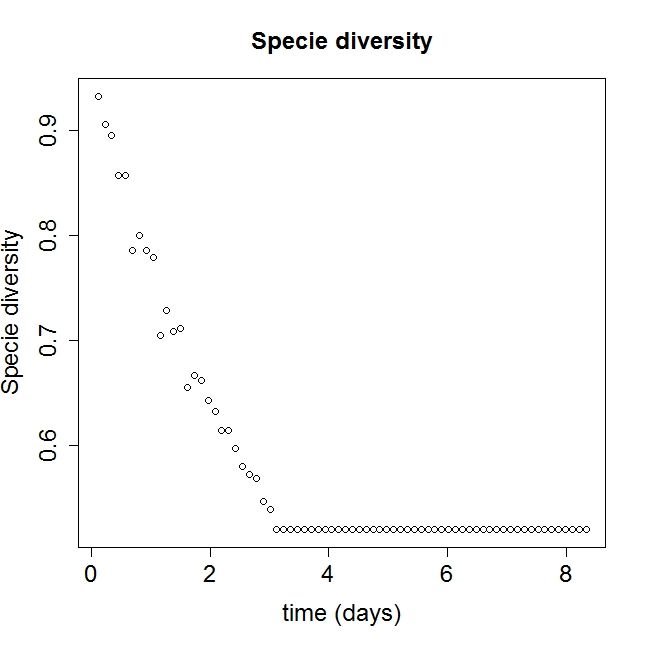
\includegraphics[width=1\textwidth]{p2/s274}
%\caption{$\lim_{\delta \to \infty}$}
\end{subfigure}\hspace*{-1.5em}
\centering
\begin{subfigure}[b]{.5\textwidth}
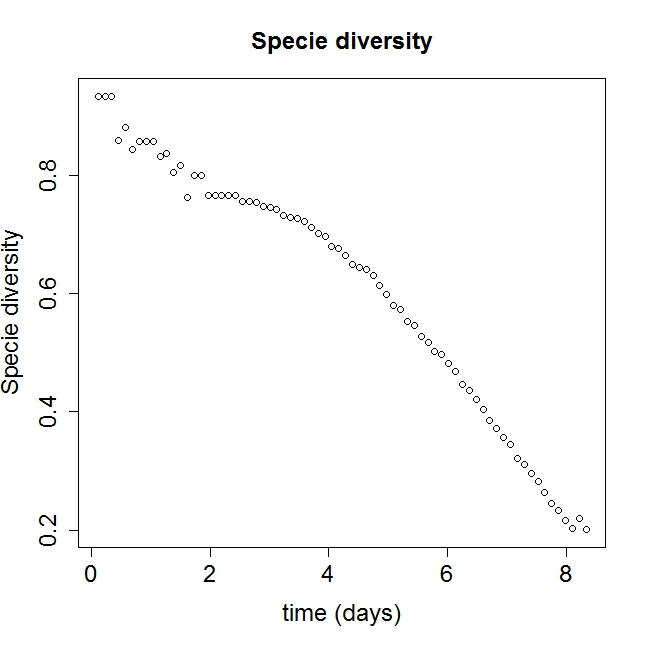
\includegraphics[width=1\textwidth]{p2/s278}%{result2/diag1bb}
%\caption{$\lim_{\delta \to 0}$}
\end{subfigure}\vspace*{-0.4em}
\begin{subfigure}[b]{.5\textwidth}
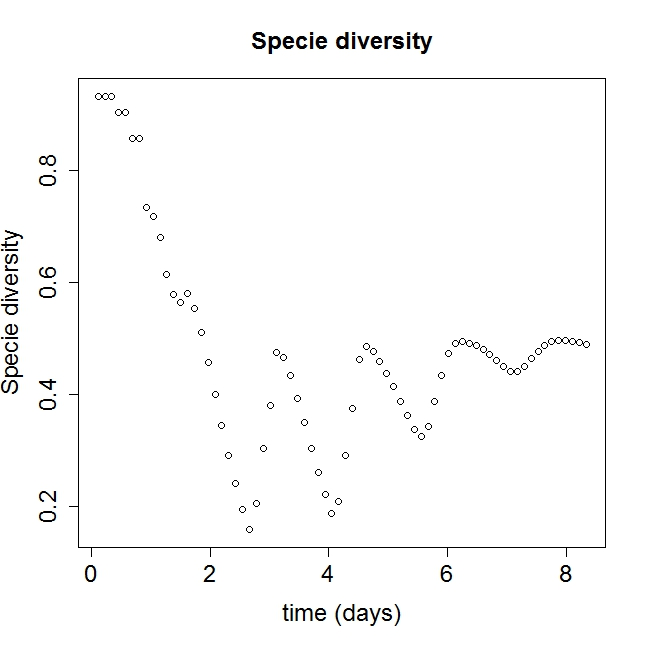
\includegraphics[width=1\textwidth]{p2/s281}
%\caption{$\lim_{\delta \to \infty}$}
\end{subfigure}\hspace*{-1.5em}
\centering
\begin{subfigure}[b]{.50\textwidth}
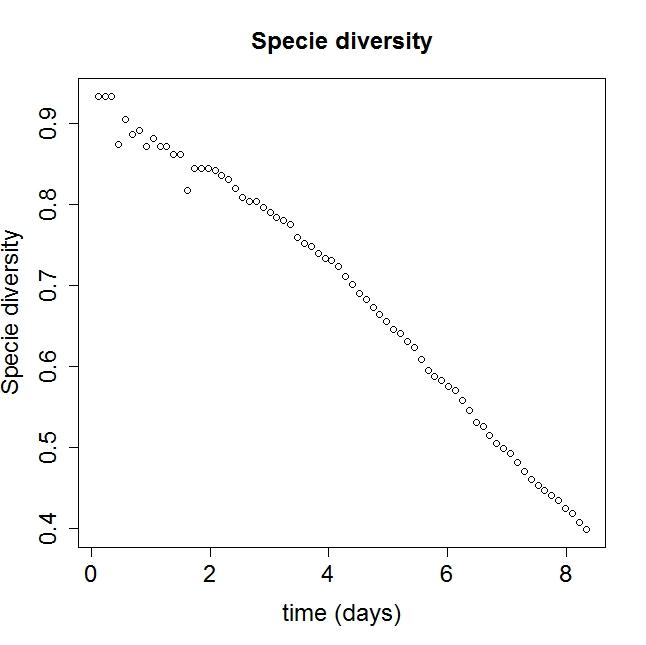
\includegraphics[width=1\textwidth]{p2/s280}
%\caption{$\lim_{\delta \to 0}$}
\end{subfigure}\vspace*{-1.5em}
\caption[]{Diverging behaviour of floc species diversity indices over time for some randomly selected design points}\label{div}
\end{figure}


\begin{figure}[!ht]
\begin{subfigure}[b]{.6\textwidth}
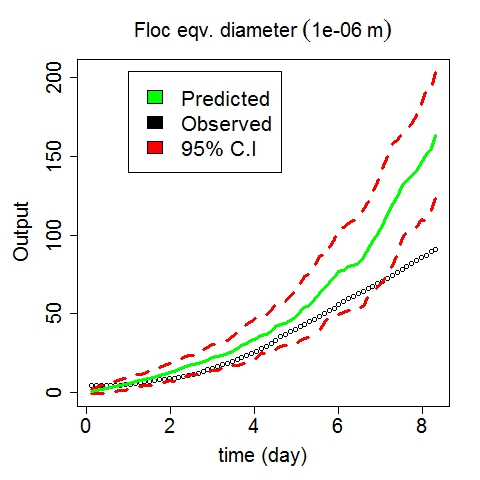
\includegraphics[width=1\textwidth]{p1d/p1d_2}
%\caption{$\lim_{\delta \to \infty}$}
\end{subfigure}\hspace*{-.5em}
\centering
\begin{subfigure}[b]{.60\textwidth}
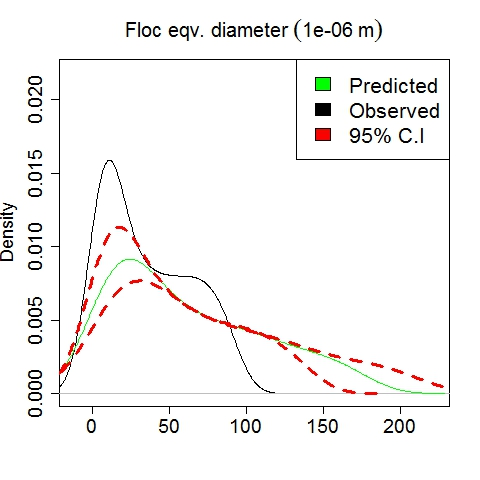
\includegraphics[width=1\textwidth]{p1a1/p1a1_2}
%\caption{$\lim_{\delta \to 0}$}
\end{subfigure}\vspace*{-.5em}
\caption[]{Comparison of time series plot and density function of floc equivalent diameter  for LAMMPS model and emulator with 95\% C.I}\label{ress3b}
\end{figure}

\end{document}